% =====================================================================
% StaticKD -- single-file manuscript (IEEEtran journal layout)
% Built by scripts/build_paper.py from src/paper/ and the notebook outputs; numbers are literal.
% results/final/paper_number_map.json lists every number; scripts/check_paper.py reports changes.
% Compile: pdflatex main && bibtex main && pdflatex main && pdflatex main
% =====================================================================
\documentclass[journal]{IEEEtran}

\usepackage[T1]{fontenc}
\usepackage[utf8]{inputenc}
\usepackage[nocompress]{cite}
\usepackage{amsmath,amssymb}
\usepackage{graphicx}
\usepackage{booktabs}
\usepackage{multirow}
\usepackage{array}
\usepackage{xcolor}
\usepackage[hyphens]{url}
\usepackage{algorithm}
\usepackage{algpseudocode}
\usepackage{tikz}
\usetikzlibrary{positioning,arrows.meta,fit,calc}

\DeclareRobustCommand{\todo}[1]{{\color{red}[TODO: #1]}}

\emergencystretch=1.5em

\begin{document}

\title{StaticKD: Mendistilasi Pengklasifikasi Topik Berita IPTC Multibahasa ke dalam Tabel Logit Token Statis untuk Inferensi CPU yang Ringan}

\author{Obi~Kastanya and Ananta~Dwi~Prayoga~Alwy%
\thanks{O. Kastanya dan A. D. P. Alwy berafiliasi dengan Departemen Teknik Informatika, Institut Teknologi Sepuluh Nopember, Surabaya, Indonesia (e-mail: 6025252015@student.its.ac.id; 6025252007@student.its.ac.id). Penulis korespondensi: O. Kastanya. Penelitian ini tidak menerima pendanaan khusus.}}

\markboth{IEEE Access (draft)}%
{Kastanya and Alwy: StaticKD, Multilingual IPTC News Topic Classification on CPU}

\maketitle

\begin{abstract}
Penyaringan berita berdasarkan taksonomi Media Topic dari International Press Telecommunications Council (IPTC) membutuhkan pengklasifikasi yang cukup murah untuk aliran artikel multibahasa. Pengklasifikasi IPTC multibahasa terbuka yang tersedia saat ini berbasis XLM-RoBERTa-large dan membutuhkan 1,239 hingga 2,971 milidetik per artikel pada satu core prosesor. Dengan pengklasifikasi ini sebagai teacher, StaticKD menyimpan 17 skor untuk setiap token dalam kosakata, satu skor untuk setiap topik IPTC tingkat atas. Klasifikasi sebuah artikel kemudian hanya memerlukan tokenisasi artikel dan perataan skor token-tokennya. Student diinisialisasi dari embedding statis multibahasa (satu vektor tetap per token) dan belajar dari keluaran teacher pada 285,999 artikel dalam 69 bahasa. Evaluasi menggunakan test set baru berisi 12,744 artikel dalam 47 bahasa. Topik artikel tersebut ditetapkan oleh annotator manusia atau editor redaksi dan dipetakan ke IPTC, sehingga tidak ada label test yang berasal dari model yang membaca artikel. Pada test set ini, StaticKD mencapai macro-F1 sebesar 0.545, atau 91.1\% dari skor teacher (0.598). Model berukuran 34 megabyte ini mengklasifikasikan 473 artikel per detik per core, sekitar 616 kali lebih cepat daripada teacher yang dikuantisasi 8-bit. Model ini juga lebih akurat daripada fastText dan linear support vector machine yang dilatih pada label teacher yang sama. Ablasi dengan lima seed menunjukkan bahwa akurasi terutama berasal dari data latih multibahasa dan embedding lintas bahasa yang sudah dilatih sebelumnya, serta bahwa label teratas dari teacher bekerja sama baiknya dengan distribusi penuh. Fine-tuning embedding merugikan bahasa yang data latihnya sedikit atau tidak ada sama sekali. StaticKD paling lemah pada bahasa yang tidak ada dalam data latihnya maupun dalam data pre-training teacher.
\end{abstract}

\begin{IEEEkeywords}
Inferensi efisien, distilasi pengetahuan, klasifikasi teks multibahasa, klasifikasi topik berita, embedding statis.
\end{IEEEkeywords}

\section{Pendahuluan}
\label{sec:introduction}
\IEEEPARstart{P}{ipeline} analitik berita membutuhkan penyaringan topik agar berita yang tidak relevan tidak diproses pada tahap-tahap berikutnya dan menambah biaya. Sebelum disaring, artikel berita harus diklasifikasikan ke dalam kategori topik standar, seperti kategori pada taksonomi Media Topic dari International Press Telecommunications Council (IPTC). Taksonomi IPTC membagi topik berita menjadi 17 kategori tingkat atas, yang memuat banyak subkategori~\cite{iptc2024mediatopics,kuzman2025llm}.

Pengklasifikasi IPTC multibahasa terbuka yang pertama dirilis oleh Kuzman dan Ljube\v{s}i\'c~\cite{kuzman2025llm}. GPT-4o digunakan untuk memberi label pada artikel dalam empat bahasa, lalu label tersebut dipakai sebagai data untuk fine-tuning XLM-RoBERTa-large~\cite{conneau2020xlmr}. Pada test set yang dianotasi manusia, model yang dihasilkan sebanding dengan GPT-4o. Studi lanjutan oleh kelompok yang sama menyimpulkan bahwa encoder hasil fine-tuning lebih praktis daripada large language model (LLM) untuk anotasi skala besar~\cite{kuzman2025southslavic}. Tanpa graphics processing unit (GPU), encoder dengan 559.9~juta parameter tetap mahal. Studi ini menyasar server tanpa GPU, tempat pengklasifikasi berbagi core central processing unit (CPU) dengan bagian pipeline lainnya. Model ini membutuhkan 2,971~ms per artikel pada satu core CPU. Konfigurasi CPU tercepatnya adalah ekspor Open Neural Network Exchange (ONNX) yang dikuantisasi ke bilangan bulat 8-bit (int8), dan konfigurasi ini pun masih membutuhkan 1,239~ms. Dengan latensi seperti itu, klasifikasi topik saja akan menghabiskan 15.1 (ONNX int8) hingga 34.8 (PyTorch) core CPU untuk aliran satu juta artikel per hari (Bagian~\ref{sec:res-eff}). Kedua studi sebelumnya tidak melaporkan biaya inferensi ini, padahal inferensi menyumbang porsi besar dari kebutuhan komputasi dan penggunaan energi machine learning di lingkungan produksi. Google, misalnya, melaporkan bahwa 60\% penggunaan energi machine learning-nya berasal dari inferensi~\cite{luccioni2024power}.

Pipeline seperti itu membutuhkan pengklasifikasi topik yang mencakup banyak bahasa dan berjalan dalam hitungan milidetik per artikel pada CPU biasa. Pengklasifikasi tersebut juga harus kecil dan memiliki sedikit dependensi. Transformer kecil hasil distilasi~\cite{sanh2019distilbert,wang2021minilmv2} memberikan percepatan sekitar satu orde besaran. Pada benchmark CPU dalam studi ini, MiniLM-L6 berjalan 21 kali lebih cepat daripada teacher ONNX int8. Kuantisasi int8 saja memberikan percepatan 2.3 kali dibandingkan PyTorch fp32. fastText~\cite{joulin2017bag} jauh lebih cepat, tetapi mempelajari vektor katanya dari nol sehingga tidak mendukung transfer lintas bahasa. Dalam kasus ini, keterbatasan tersebut serius. Label latih IPTC yang dirilis bersama pengklasifikasi terbuka hanya mencakup empat bahasa~\cite{emmediatopic2025}. Bahkan korpus yang dilabeli secara otomatis oleh teacher multibahasa tidak mungkin memuat semua bahasa dalam aliran berita. Tidak satu pun pengklasifikasi IPTC yang tersedia sekaligus multibahasa dan semurah ini.

Metode StaticKD yang diusulkan dalam makalah ini mendistilasi~\cite{hinton2015distilling} pengklasifikasi IPTC XLM-R-large ke dalam student yang jauh lebih sederhana. Tiga sifat masalah ini membuatnya mungkin dilakukan. Berita tanpa label dalam bahasa apa pun dapat dilabeli oleh teacher yang bekerja lintas bahasa, sehingga data latih untuk student tidak memerlukan biaya anotasi. Embedding statis multibahasa yang didistilasi dari sentence encoder~\cite{tulkens2024model2vec,wada2025static,chen2024bgem3} memberi setiap token satu vektor tetap dan menempatkan padanan terjemahan saling berdekatan. Mencari vektor semacam itu hampir tidak membutuhkan biaya. Topik berita juga terkait erat dengan kosakata, yang menjelaskan mengapa representasi bag-of-words tetap kompetitif untuk klasifikasi topik~\cite{galke2022bow}. Karena itu, student merata-ratakan embedding token dalam sebuah artikel lalu menerapkan satu lapisan linear. Kedua langkah ini linear, sehingga lapisan linear dapat diterapkan satu kali pada setiap embedding sebelum deployment. Penerapan lapisan sebelum deployment ini disebut folding dalam makalah ini. Folding mengubah model menjadi tabel yang menyimpan 17 skor topik (logit) per token. Klasifikasi sebuah artikel kemudian cukup dengan tokenisasi dan perataan baris tabel dari token-tokennya. Komputasi berjalan di NumPy tanpa pustaka deep learning. Gambar~\ref{fig:tradeoff} pada Bagian~\ref{sec:res-eff} membandingkan akurasi dan kecepatan StaticKD dengan model lainnya.

Klaim multibahasa juga memerlukan evaluasi multibahasa dengan label yang tidak berasal dari teacher. Test set beranotasi manusia milik Kuzman dan Ljube\v{s}i\'c tidak dipublikasikan dan hanya mencakup empat bahasa. SIB-200~\cite{adelani2024sib200} mencakup 205 bahasa, tetapi itemnya berupa kalimat pendek dan taksonominya bukan IPTC. Studi ini mengisi celah tersebut dengan membangun test set terpadu berisi 12,744 artikel dalam 47 bahasa. Sebagian artikelnya adalah halaman berita tahun 2024 hingga 2026 yang penerbitnya mencatat rubrik redaksi artikel pada metadata halaman (schema.org~\cite{guha2016schema}). Halaman-halaman tersebut digabungkan dengan dataset publik yang dilabeli oleh annotator manusia atau dengan kategori penerbit~\cite{adelani2023masakhanews,petukhova2023mnds,mirashi2023indicnews,hossain2025banglanews}. Setiap label merupakan keputusan editorial penerbit atau annotator yang kemudian dipetakan ke taksonomi resmi IPTC. Prosesnya tidak melibatkan model yang membaca teks artikel.

Studi ini menjawab empat research question (RQ). RQ1 menanyakan seberapa besar akurasi teacher yang dipertahankan StaticKD pada label yang tidak berasal dari teacher. Perbandingan menggunakan dua baseline dengan biaya serupa, yaitu fastText dan support vector machine (SVM) dengan fitur term frequency--inverse document frequency (TF-IDF). Model lain dalam perbandingan adalah MiniLM-L6 dan DistilmBERT, dua transformer kecil yang lebih mahal. RQ2 menelaah bagian mana dari resep pelatihan yang berpengaruh untuk student yang sangat kecil ini. Bagian yang diuji adalah soft label, data multibahasa, inisialisasi embedding, fine-tuning embedding, token dropout, temperature, dan ensembling. Untuk RQ3, studi ini mengukur biaya inferensi teacher pada CPU dan seberapa jauh StaticKD menurunkan biaya tersebut. RQ4 mencari bahasa, label, dan sumber label yang menjadi kelemahan StaticKD, beserta faktor di balik kelemahan tersebut.

Jawaban RQ2 dan RQ4 menunjukkan bahwa akurasi StaticKD bergantung pada banyaknya bahasa dan situs yang dicakup data berlabel teacher serta pada apakah embedding dimulai dari ruang yang dipakai bersama oleh semua bahasa. Melatih student hanya dengan label teratas teacher memberikan hasil sebaik melatihnya dengan distribusi penuh teacher. Fine-tuning embedding membantu pada dev set tetapi merugikan bahasa yang data distilasinya sedikit atau tidak ada. Dev set dalam bahasa-bahasa latih tidak dapat memperlihatkan trade-off ini.

Kontribusi makalah ini adalah sebagai berikut.
\begin{enumerate}
  \item StaticKD, sebuah resep yang mendistilasi teacher transformer multibahasa ke dalam tabel 17 logit per token, yang diinisialisasi dari embedding statis multibahasa. Model akhir berukuran 34~MB dan hanya membutuhkan pustaka \texttt{numpy} dan \texttt{tokenizers}. Model ini memproses 473 artikel per detik per core. Ensemble dari beberapa student terlatih dilipat (fold) ke dalam satu tabel yang sama, sehingga tidak menambah biaya inferensi.
  \item Test set IPTC multibahasa berisi 12,744 artikel dalam 47 bahasa, dengan label editorial yang tidak berasal dari teacher. Test set ini dilengkapi tabel pemetaan rubrik-ke-IPTC yang diperiksa secara otomatis dan ditinjau oleh penulis pertama. Duplikat antarsumber telah dihapus, dan kontaminasi telah diperiksa terhadap seluruh data latih. Confidence interval memperhitungkan bahwa artikel dari situs yang sama saling berkaitan. Pengklasifikasi IPTC lain dapat dievaluasi pada test set yang sama.
  \item Temuan di atas tentang asal akurasi student, didukung oleh ablasi dengan lima seed per varian. Dukungan lebih lanjut berasal dari analisis per bahasa, label, asal label, dan dataset sumber. Bahasa yang tidak ada dalam data latih juga dianalisis. Akurasi dan biaya diukur hanya pada CPU untuk sembilan konfigurasi dari enam keluarga model, termasuk StaticKD. Setiap proses dipatok (pinned) pada core cepat dari CPU hibrida.
  \item Rilis kode, notebook yang mereproduksi setiap angka dalam makalah ini, model, dan manifest test set.
\end{enumerate}

Bagian~\ref{sec:related} mengulas penelitian terkait. Data, test set, metode, dan protokol evaluasi dijelaskan pada Bagian~\ref{sec:method}. Hasil disajikan pada Bagian~\ref{sec:results} dan dibahas pada Bagian~\ref{sec:discussion}. Bagian~\ref{sec:limitations} menyatakan keterbatasan studi, dan Bagian~\ref{sec:conclusion} menutup makalah ini.

\section{Penelitian Terkait}
\label{sec:related}
\subsection{Klasifikasi Topik Berita Multibahasa dan Skema IPTC}
Dataset untuk klasifikasi topik berita biasanya mendefinisikan taksonominya sendiri dan hanya mencakup satu bahasa atau satu wilayah. Pada MasakhaNEWS~\cite{adelani2023masakhanews}, annotator manusia melabeli artikel berita dengan tujuh kategori. Dataset ini mencakup 16 bahasa yang banyak digunakan di Afrika, termasuk Inggris dan Prancis. Dua dataset lain mengambil label dari kategori situs penerbit, yaitu L3Cube-IndicNews untuk 10 bahasa India~\cite{mirashi2023indicnews} dan dataset berita Bangla~\cite{hossain2025banglanews}. Di antara dataset publik, hanya MN-DS~\cite{petukhova2023mnds} yang dianotasi langsung dengan topik IPTC tingkat atas. Artikelnya hanya berbahasa Inggris. SIB-200~\cite{adelani2024sib200} mencakup 205 bahasa, tetapi datanya berupa kalimat Flores-200 dengan tujuh topik non-IPTC. Kuzman dan Ljube\v{s}i\'c~\cite{kuzman2025llm} menunjukkan bahwa label GPT-4o dapat menggantikan anotasi manusia untuk melatih pengklasifikasi IPTC. Studi lanjutan mereka menemukan bahwa encoder hasil fine-tuning lebih praktis daripada LLM untuk anotasi skala besar~\cite{kuzman2025southslavic}. Satu-satunya pengklasifikasi IPTC multibahasa terbuka adalah encoder dengan 559.9~juta parameter. Belum ada pengklasifikasi IPTC murah yang dievaluasi pada berita nyata dalam banyak bahasa.

\subsection{Mendistilasi Pengklasifikasi Transformer ke dalam Student yang Ringkas}
Knowledge distillation (KD) melatih model student yang murah untuk meniru distribusi keluaran model teacher yang mahal~\cite{hinton2015distilling,yang2025kdsurvey}. Sebelum softmax, vektor logit teacher dan student sama-sama dibagi dengan temperature $\tau$. $\tau$ yang lebih tinggi membuat distribusi lebih datar, sehingga student juga mempelajari seberapa besar probabilitas yang diberikan teacher pada kelas yang salah. Distribusi penuh disebut soft label, sedangkan kelas teratasnya saja disebut hard label. Pada klasifikasi teks, student hampir selalu berupa transformer seperti DistilBERT~\cite{sanh2019distilbert} atau MiniLMv2~\cite{wang2021minilmv2}. Hal yang sama berlaku untuk distilasi lintas bahasa yang mentransfer pengetahuan teacher ke bahasa dengan data sedikit~\cite{piperno2025crosslingual}. Karya terdahulu yang paling dekat dengan StaticKD adalah Sparse Distillation~\cite{ye2022sparse}. Karya ini mendistilasi RoBERTa-large ke dalam deep averaging network~\cite{iyyer2015dan} dengan tabel n-gram yang sangat besar. Pada tugas klasifikasi kalimat tunggal berbahasa Inggris, model yang dihasilkan berjalan ratusan kali lebih cepat. StaticKD berbeda dari Sparse Distillation dalam tiga hal. Tabelnya tidak dilatih dari nol, melainkan dimulai dari embedding statis multibahasa yang sudah selaras lintas bahasa. Setiap token hanya menyimpan 17 angka karena linear head dilipat. StaticKD menyasar dokumen berita dalam 69 bahasa, dan evaluasinya juga mencakup bahasa yang tidak ada dalam data distilasi.
\subsection{Temperature dan Kesenjangan Kapasitas}
Keberhasilan distilasi bergantung pada kesenjangan kapasitas antara teacher dan student. Kesenjangan ini melebar ketika teacher menjadi lebih besar dan lebih ekspresif daripada student. Untuk model bahasa, ukuran teacher yang optimal bahkan mengikuti hukum empiris terhadap ukuran student~\cite{zhang2025law}. Temperature diperlakukan sebagai hyperparameter penting yang dapat dipelajari~\cite{li2023ctkd}. Kullback--Leibler (KL) divergence dapat dipecah menjadi bagian kelas target dan bagian non-target (dark knowledge)~\cite{zhao2022dkd}. Sebuah analisis terbaru~\cite{wang2026rckd} menunjukkan bahwa KL mendistorsi peringkat kelas ketika kapasitas teacher dan student tidak cocok. Temuan lain adalah bahwa generalisasi tidak selalu membaik ketika kesesuaian antara student dan teacher (fidelity) tinggi~\cite{stanton2021kd}. Hampir semua temuan ini berasal dari student yang dalam. Belum ada studi yang mengkarakterisasi perilaku temperature dan soft label pada kesenjangan ekstrem, yaitu dari 559.9~juta parameter menjadi satu lapisan linear di atas embedding yang dirata-ratakan.

\subsection{Embedding Statis dan Inferensi CPU yang Efisien}
Embedding statis memberi setiap token satu vektor tetap yang tidak bergantung pada kata-kata di sekitarnya, sehingga vektor sebuah teks hanyalah rata-rata vektor token-tokennya. Embedding semacam itu diekstrak dari sentence transformer oleh Model2Vec~\cite{tulkens2024model2vec} dan oleh Wada dkk.~\cite{wada2025static}. Rata-rata embedding ini merupakan sentence embedding yang kompetitif. Model2Vec memiliki varian multibahasa bernama potion-multilingual, yang didistilasi dari BGE-M3~\cite{chen2024bgem3} dan mencakup 101 bahasa. Pustaka Model2Vec juga menyediakan trainer pengklasifikasi yang menambahkan hidden layer 512 unit dan belajar dari hard label~\cite{tulkens2024model2vec}. Embedding statis biasanya dievaluasi sebagai embedding serbaguna, bukan sebagai student distilasi untuk taksonomi tertentu. Sebuah survei metode natural language processing (NLP) yang efisien merekomendasikan pelaporan biaya inferensi bersama akurasi~\cite{treviso2023efficient}, karena inferensi menyumbang porsi besar dari penggunaan energi model yang dideploy~\cite{luccioni2024power}. Namun, hanya sedikit studi yang melaporkan latensi CPU pada jumlah thread rendah dengan teacher terkuantisasi sebagai pembanding.

\subsection{Test Set dengan Label Editorial, Kontaminasi, dan Ketergantungan Sampel}
Kategori situs penerbit pernah digunakan sebagai label topik sebelumnya~\cite{mirashi2023indicnews}, biasanya untuk satu penerbit atau satu wilayah. Banyak situs berita juga mencatat rubrik setiap artikel dalam metadata halaman yang dapat dibaca mesin, yaitu bidang \texttt{articleSection} dari schema.org~\cite{guha2016schema}. Hingga kini, bidang tersebut belum dipetakan ke taksonomi standar lintas puluhan bahasa. Kebocoran antara data latih dan data uji juga harus dikendalikan. Penghapusan near-duplicate dengan MinHash~\cite{broder1997resemblance} telah menjadi praktik standar~\cite{lee2022dedup}. Dalam NLP, uji signifikansi seperti paired bootstrap~\cite{koehn2004significance} biasanya mengasumsikan sampel independen~\cite{dror2018hitchhiker}, sedangkan artikel dari situs yang sama saling bergantung. Cluster bootstrap~\cite{field2007bootstrapping} menangani ketergantungan ini dengan melakukan resampling pada klaster, bukan pada dokumen. Posisi StaticKD relatif terhadap pendekatan-pendekatan ini diringkas pada Tabel~\ref{tab:related}.

\begin{table*}[!t]
\caption{Position of StaticKD Relative to Related Approaches}
\label{tab:related}
\centering
\footnotesize
\setlength{\tabcolsep}{4pt}
\resizebox{\textwidth}{!}{%
\begin{tabular}{@{}llccccc@{}}
\toprule
Approach & Model at inference time & Multilingual & Cross-lingual transfer & No deep learning library & CPU cost reported & IPTC labels \\
\midrule
Kuzman \& Ljube\v{s}i\'c~\cite{kuzman2025llm} & XLM-R-large (559.9M parameters) & yes & yes & no & no & yes \\
DistilBERT, MiniLMv2~\cite{sanh2019distilbert,wang2021minilmv2} & 6-layer transformer & partly & yes & no & partly & no \\
Sparse Distillation~\cite{ye2022sparse} & deep averaging network + n-gram table & no (en) & no & yes & yes & no \\
Model2Vec~\cite{tulkens2024model2vec}, Wada et al.~\cite{wada2025static} & static embeddings, optional MLP classifier & yes & yes & yes & partly & no \\
fastText~\cite{joulin2017bag} & bag of n-grams & per language & no & yes & yes & no \\
StaticKD (proposed) & table of 17 logits per token & yes & yes & yes & yes & yes \\
\bottomrule
\end{tabular}}
\end{table*}

\section{Metodologi}
\label{sec:method}
\subsection{Desain Penelitian}
Penelitian ini terdiri atas tiga tahap utama: membangun student StaticKD melalui distilasi, mengukur dan membandingkan akurasi pada artikel berlabel yang belum pernah dilihat oleh teacher maupun student, serta mengukur biaya inferensi di CPU.

Gambar~\ref{fig:pipeline} menunjukkan pipeline StaticKD yang dibangun dalam penelitian ini. Teacher mengklasifikasikan 285,999 artikel tak berlabel dalam 69 bahasa dan menghasilkan logit untuk 17 topik IPTC tingkat atas (Bagian~\ref{sec:distdata} dan~\ref{sec:teacher}). Logit adalah skor mentah yang dikeluarkan model untuk setiap kelas sebelum diubah menjadi probabilitas. Model StaticKD dilatih untuk meniru distribusi teacher atas 17 topik IPTC tersebut (Bagian~\ref{sec:student}). Baseline berbasis transformer (MiniLM-L6 dan DistilmBERT) dilatih dengan gradient descent seperti StaticKD dan memakai loss yang sama pada distribusi penuh. fastText dan TF-IDF + SVM hanya belajar dari label teratas teacher, karena prosedur pelatihan standarnya hanya menerima satu kelas per dokumen. Satu model fastText tambahan dilatih dengan label GPT-4o dari dataset EMMediaTopic~\cite{emmediatopic2025}, yang dirilis bersama teacher. Model ini menguji seberapa baik classifier murah bekerja tanpa label teacher pada berita multibahasa (Bagian~\ref{sec:baselines}).

Penelitian ini tidak memakai label hasil prediksi teacher sebagai ground truth. Kecocokan yang tinggi antara skor student dan teacher hanya menunjukkan seberapa dekat student meniru teacher. Akurasi prediksi dievaluasi pada test set terpisah (Bagian~\ref{sec:testset}). Test set tersebut mengelompokkan artikel berita menurut label editorial aslinya, yang diambil dari informasi seperti kolom section dan breadcrumb pada metadata schema.org JSON-LD setiap halaman. Sebuah LLM dipakai untuk memetakan label editorial ke 17 topik IPTC, dan artikel dengan kategori yang ambigu dikeluarkan. Penulis pertama kemudian meninjau pemetaan ini. Tahap ketiga menjalankan setiap model hanya di CPU, dengan sampel artikel uji yang sama. Bagian~\ref{sec:effprotocol} menjelaskan benchmark ini.

Tabel~\ref{tab:datasets} mendaftar dataset yang dipakai dalam penelitian ini. Semua pengaturan parameter dan pilihan resep StaticKD ditetapkan pada dev set, yaitu split pengembangan dari EMMediaTopic (1,000 artikel dalam empat bahasa dengan label GPT-4o). Resep tersebut ditetapkan \emph{sebelum} test set dibangun. Satu set lain juga ikut menjadi dasar bagi dua dari pilihan ini: temperature $\tau=1$ dan ensemble tiga seed (Bagian~\ref{sec:student}). Set ini berisi 320 artikel dalam 16 bahasa yang dilabeli oleh sebuah LLM (Claude) dengan prompt dari~\cite{kuzman2025llm}. Teacher dilatih dengan label yang dihasilkan sebuah LLM (GPT-4o) dengan prompt yang sama, sehingga label ini tidak independen dari teacher. Tidak ada hasil yang dilaporkan yang memakai set ini.

\begin{table}[!t]
\caption{Data Sets of the Study and Their Roles}
\label{tab:datasets}
\centering
\footnotesize
\setlength{\tabcolsep}{3pt}
\resizebox{\columnwidth}{!}{%
\begin{tabular}{@{}lrrll@{}}
\toprule
Set & Docs & Lang. & Labels & Used for \\
\midrule
Distillation data & 285,999 & 69 & teacher & training the students \\
\quad internal validation & 8,579 & -- & teacher & choosing the epoch \\
Development (EMMediaTopic) & 1,000 & 4 & GPT-4o & choosing the recipe \\
CC-News held-out & 12,554 & 63 & teacher & agreement, unseen sites \\
Unified test set & 12,744 & 47 & editorial & all accuracy results \\
LLM check set & 320 & 16 & Claude & informal check only \\
English section sample & 754 & 1 & JSON-LD & label validity only \\
\bottomrule
\end{tabular}}
\end{table}

\begin{figure*}[!t]
\centering
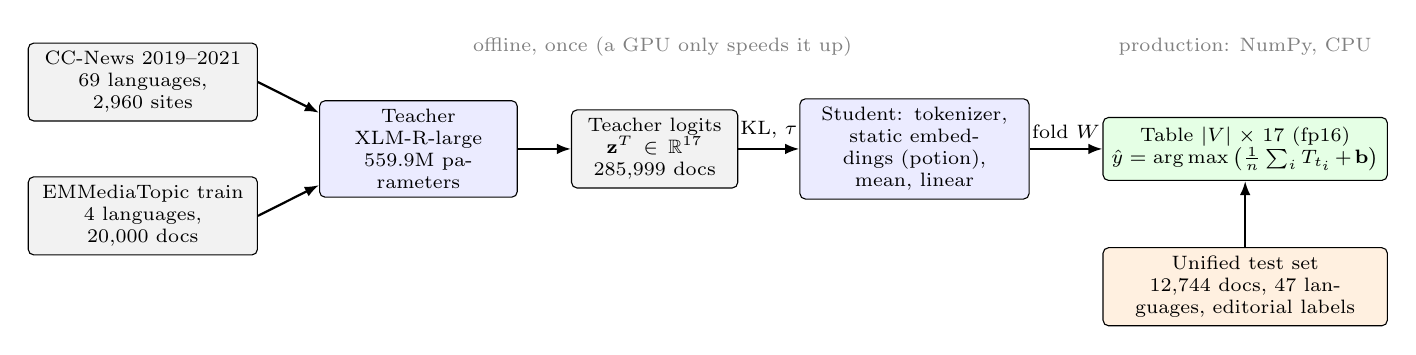
\begin{tikzpicture}[
  box/.style={draw, rounded corners=2pt, align=center, font=\scriptsize, inner sep=3pt, minimum height=8mm},
  data/.style={box, fill=gray!10},
  model/.style={box, fill=blue!8},
  prod/.style={box, fill=green!10},
  test/.style={box, fill=orange!12},
  arr/.style={-{Latex[length=1.8mm]}, thick},
  lab/.style={font=\scriptsize}]
  \node[data, text width=27mm] (cc)  at (1.4, 0.85)  {CC-News 2019--2021\\69 languages, 2,960 sites};
  \node[data, text width=27mm] (emm) at (1.4,-0.85)  {EMMediaTopic train\\4 languages, 20,000 docs};
  \node[model, text width=23mm] (t)  at (4.9, 0)     {Teacher\\XLM-R-large\\559.9M parameters};
  \node[data, text width=19mm] (soft) at (7.9, 0)    {Teacher logits\\$\mathbf{z}^{T}\in\mathbb{R}^{17}$\\285,999 docs};
  \node[model, text width=27mm] (s)  at (11.2, 0)    {Student: tokenizer,\\static embeddings (potion),\\mean, linear};
  \node[prod, text width=34mm] (tab) at (15.4, 0)    {Table $|V|\times 17$ (fp16)\\$\hat{y}=\arg\max\big(\frac{1}{n}\sum_i T_{t_i}+\mathbf{b}\big)$};
  \node[test, text width=34mm] (ts) at (15.4, -1.75)  {Unified test set\\12,744 docs, 47 languages, editorial labels};
  \draw[arr] (cc.east)  -- (t.160);
  \draw[arr] (emm.east) -- (t.200);
  \draw[arr] (t) -- (soft);
  \draw[arr] (soft) -- node[lab, above]{KL, $\tau$} (s);
  \draw[arr] (s) -- node[lab, above]{fold $W$} (tab);
  \draw[arr] (ts.north) -- (tab.south);
  \node[lab, text=gray] at (8.0, 1.3) {offline, once (a GPU only speeds it up)};
  \node[lab, text=gray] at (15.4, 1.3) {production: NumPy, CPU};
\end{tikzpicture}
\caption{StaticKD pipeline. The teacher labels an unlabeled news corpus once, offline. The student learns to imitate the teacher distribution, and its linear head is then folded into a token table, so inference only looks up and averages table rows. The final evaluation uses a test set whose labels do not come from the teacher.}
\label{fig:pipeline}
\end{figure*}

\subsection{Formulasi Masalah}
Diberikan sebuah artikel berita $d$ dalam bahasa apa pun (judul dan isi, dipotong menjadi 512 kata pertama seperti pada~\cite{kuzman2025llm}), sebuah model memprediksi satu label $y\in\mathcal{Y}$ di antara 17 topik IPTC tingkat atas. Teacher $f_T$ menghasilkan logit $\mathbf{z}^T(d)\in\mathbb{R}^{17}$. Tujuannya adalah student $f_S$ yang biaya inferensinya $O(n)$ penjumlahan untuk $n$ token dan tidak memerlukan perkalian matriks maupun library deep learning. Akurasinya terhadap label independen harus sedekat mungkin dengan akurasi $f_T$.

\subsection{Data Distilasi dan Dev Set}
\label{sec:distdata}
Data distilasi dan dev set sama-sama bersumber dari EMMediaTopic 1.0~\cite{emmediatopic2025,kuzman2025llm}, yang dirilis oleh Kuzman dan Ljube\v{s}i\'c bersama model teacher. EMMediaTopic dilabeli dengan GPT-4o dan terdiri atas artikel dalam empat bahasa (Katalan, Yunani, Kroasia, dan Slovenia). Dari anotasi tersebut, 21,000 artikel diambil dan dibagi menjadi split pelatihan sebanyak 20,000 artikel dan split pengembangan sebanyak 1,000 artikel. Split pelatihan adalah data yang dipakai Kuzman dan Ljube\v{s}i\'c untuk melatih teacher, dan penelitian ini memakainya sebagai bagian dari data distilasi untuk student. Split pengembangan tidak pernah dipakai untuk melatih teacher maupun student. Split ini dipakai untuk mencari hyperparameter teacher~\cite{kuzman2025llm}, dan penelitian ini memakainya sebagai dev set untuk memilih resep StaticKD.

Sebagian besar data distilasi berasal dari CC-News 2019--2021, dataset multibahasa~\cite{cloversearch_ccnews} yang dibangun dari arsip berita Common Crawl. Sebaliknya, test set diambil dari CC-News untuk rentang tahun yang berbeda (CC-NEWS 2024--2026, Bagian~\ref{sec:testset}). CC-News 2019--2021 diproses dengan langkah-langkah berikut.
\begin{enumerate}
  \item Memverifikasi bahasa dengan model identifikasi bahasa fastText~\cite{joulin2017bag} dan hanya mempertahankan dokumen yang bahasa pada metadata-nya sesuai dengan bahasa hasil identifikasi.
  \item Mengambil judul dan isi jika totalnya minimal 75 kata (200 karakter untuk ja, zh, th, my), lalu memotongnya menjadi 512 kata.
  \item Mempertahankan paling banyak 150 dokumen per situs.
  \item Membentuk split held-out berdasarkan domain: semua dokumen dari beberapa situs disisihkan, dengan paling banyak 20\% per bahasa.
  \item Menambahkan 156,157 dokumen hanya dari situs pelatihan (paling banyak 5,000 per bahasa dan 400 per situs).
\end{enumerate}
Data distilasi berisi 285,999 dokumen dalam 69 bahasa dari 2,960 situs, dengan median 269 kata. Jumlah dokumen per situs dibatasi untuk menghindari bias dari konten yang mirip dalam satu situs. Beberapa situs multibahasa (misalnya bbc.com) disisihkan dalam satu bahasa tetapi juga muncul dalam data distilasi pada bahasa lain, sehingga artikelnya dihapus dari split held-out. Set held-out yang dihasilkan berisi 12,554 dokumen dalam 63 bahasa dari 217 situs yang tidak pernah muncul dalam data distilasi. Set ini tidak memiliki label kategori independen, sehingga hanya dapat mengukur \emph{agreement} dengan teacher. Agreement adalah proporsi dokumen yang label prediksi teratasnya sama dengan label teratas teacher.

\subsection{Pembangunan Unified Test Set}
\label{sec:testset}
Sumber pertama adalah dataset CC-NEWS 2024--2026, yang disampel sebagai satu file arsip (WARC) per bulan dari Januari 2024 hingga Agustus 2026 (32 file)~\cite{commoncrawl2026ccnews}. Dari setiap halaman artikel, blok schema.org JSON-LD~\cite{guha2016schema} menyediakan kolom metadata seperti \texttt{articleSection}, \texttt{BreadcrumbList}, \texttt{inLanguage}, \texttt{datePublished}, \texttt{isAccessibleForFree}, dan \texttt{articleBody}. Teks diambil dari \texttt{articleBody} hanya jika panjangnya minimal 30 kata. Jika tidak, teks diekstraksi dari konten HTML dengan library Trafilatura~\cite{barbaresi2021trafilatura}. Artikel dari situs yang sudah ada dalam data distilasi atau dalam suatu set evaluasi dihapus, sehingga tersisa 399,468 artikel dari situs baru.

Sumber kedua adalah dataset publik. MasakhaNEWS~\cite{adelani2023masakhanews} dan MN-DS~\cite{petukhova2023mnds} dilabeli oleh manusia. L3Cube-IndicNews (split LDC)~\cite{mirashi2023indicnews}, Bangla news~\cite{hossain2025banglanews}, dan IndoNews~\cite{indonews2021} membawa kategori dari penerbit.

Label section dan kategori mencatat di mana redaksi menempatkan sebuah artikel saat dipublikasikan. Label semacam ini disebut \emph{label editorial} dalam makalah ini. Label editorial tidak mengikuti standar IPTC, sehingga nama section harus diterjemahkan ke pohon IPTC Media Topic resmi (1,085 node aktif). Prosesnya dimulai dengan menormalkan nama section (huruf besar/kecil, diakritik) dan dilanjutkan dengan pemetaan konservatif oleh sebuah LLM (Claude Opus 5.5). Sebuah nama dipetakan hanya jika konten di bawah section tersebut cocok dengan satu topik tingkat atas. Hasilnya, 814 nama section terpetakan ke 79 node IPTC. Pemeriksaan otomatis memverifikasi bahwa setiap node tujuan ada di pohon IPTC, tidak dinonaktifkan, dan berada di bawah topik tingkat atas yang dimaksud. Artikel yang section-nya terpetakan ke label berbeda ditolak. Penulis pertama kemudian meninjau setiap aturan pada tabel pemetaan yang dirancang oleh LLM untuk memastikan akurasinya. Peninjauan ini mencakup 916 aturan, yaitu 814 nama terpetakan yang valid dan 102 aturan yang ambigu, spesifik bahasa, dan penolakan.

Filter kualitas dan kebocoran diterapkan secara berurutan.
\begin{enumerate}
  \item Tanggal publikasi pada atau setelah 1 Januari 2024 (hanya CC-NEWS).
  \item Tidak berada di balik paywall.
  \item Bahasa yang dideklarasikan sesuai dengan identifikasi bahasa fastText jika fastText mendukung bahasa tersebut.
  \item Minimal 75 kata.
  \item Deduplikasi uniform resource locator (URL), teks identik, dan near-duplicate (MinHash~\cite{broder1997resemblance}, Jaccard $\ge 0.7$~\cite{lee2022dedup}) di seluruh sumber.
  \item Kontaminasi: sebuah artikel dibuang jika $\ge 30\%$ dari 8-gram katanya muncul di salah satu dari sekitar 300 ribu dokumen pelatihan atau evaluasi. Filter ini menghapus 50 artikel, sebagian besar dari MasakhaNEWS, yang juga mengambil dari BBC.
\end{enumerate}

Pengambilan sampel mengambil paling banyak 50 artikel untuk setiap pasangan bahasa dan label. Sumber berlabel manusia diprioritaskan, diikuti kategori penerbit, lalu section JSON-LD. Jumlah artikel per situs tidak dibatasi. Bahasa dengan kurang dari 30 artikel dibuang. Artikel dari situs yang sama cenderung mirip, sehingga seluruh situs disampel ulang saat interval kepercayaan dihitung (Bagian~\ref{sec:protocol}). Bagian~\ref{sec:res-acc} juga mengulangi perbandingan dengan paling banyak lima artikel per situs.

Test set akhir berisi 12,744 artikel dalam 47 bahasa dari 1,227 situs atau sumber. Seluruh 17 label muncul di dalamnya, dan median panjang artikel adalah 313 kata. Anotator manusia melabeli 4,094 dari artikel ini (32.1\%). Kategori penerbit mencakup 2,600 (20.4\%) dan section JSON-LD 6,050 (47.5\%). Jenis label sebuah artikel (anotasi manusia, kategori penerbit, atau section JSON-LD) disebut \emph{asal label}-nya. Tidak ada data distilasi untuk 13 bahasa (misalnya ha, yo, ig, bn, dan pa). Sembilan bahasa lain memiliki kurang dari 500 dokumen distilasi, dan 25 bahasa memiliki minimal 500. Keragaman situs diukur dengan jumlah efektif situs, $1/\sum_s q_s^{2}$, dengan $q_s$ adalah proporsi artikel suatu bahasa yang berasal dari situs $s$. Dataset sumber tanpa URL dihitung sebagai satu situs. Menurut ukuran ini, 13 bahasa memiliki minimal 10 situs efektif, sedangkan 27 bahasa praktis hanya berasal dari satu penerbit. Tabel~\ref{tab:testset} merangkum komposisi sumber artikel dan Gambar~\ref{fig:testset} menunjukkan jumlah artikel setiap bahasa per label.

\begin{table}[!t]
\caption{Composition of the Unified Test Set by Source}
\label{tab:testset}
\centering
\footnotesize
\setlength{\tabcolsep}{3pt}
\resizebox{\columnwidth}{!}{%
\begin{tabular}{@{}llrrr@{}}
\toprule
Source & Label origin & Articles & Languages & Sites/sources \\
\midrule
CC-NEWS 2024--2026 & JSON-LD section & 6,050 & 29 & 1,092 \\
MasakhaNEWS~\cite{adelani2023masakhanews} & human annotation & 3,339 & 16 & 6 \\
L3Cube-IndicNews~\cite{mirashi2023indicnews} & publisher category & 2,361 & 10 & 1 \\
MN-DS~\cite{petukhova2023mnds} & human annotation & 755 & 1 & 127 \\
Bangla news~\cite{hossain2025banglanews} & publisher category & 139 & 1 & 1 \\
IndoNews & publisher category & 100 & 1 & 1 \\
\midrule
Total & & 12,744 & 47 & 1,227 \\
\bottomrule
\end{tabular}}
\end{table}

\begin{figure}[!t]
\centering
\includegraphics[width=\columnwidth]{figures/fig_testset_heatmap.pdf}
\caption{Articles in the unified test set per language and label (at most 50 per language--label pair). The label origin in brackets is the dominant one for that language.}
\label{fig:testset}
\end{figure}

\subsection{Teacher dan Label Distilasi}
\label{sec:teacher}
Teacher adalah classifier IPTC dari~\cite{kuzman2025llm}, yang dipublikasikan sebagai \url{classla/multilingual-IPTC-news-topic-classifier}. Model ini adalah XLM-RoBERTa-large dengan 24 layer, 559.9 juta parameter, dan batas input 512 token XLM-R. Pada 60.7\% artikel uji, input 512 kata melampaui batas ini. Pada artikel-artikel tersebut teacher membaca sekitar 287 dari 438 kata (median). Untuk setiap dokumen distilasi, teacher menghasilkan vektor logit $\mathbf{z}^{T}(d)\in\mathbb{R}^{17}$, yang disimpan secara utuh. Pelabelan dijalankan satu kali dalam fp16 pada GPU NVIDIA RTX~4050 Laptop (6~GB), dengan batch yang diurutkan menurut panjang teks. Berdasarkan pengukuran pada sampel tetap 5,000 dokumen, teacher melabeli 50.1 dokumen per detik, sehingga pelabelan seluruh data distilasi memakan waktu sekitar 1.58 jam GPU. Distribusi label teacher pada CC-News 2019--2021 tampak masuk akal (\emph{politics} 16.5\%, \emph{economy} 12.7\%, \emph{sport} 11.6\%, \emph{weather} 1.3\%), dan rata-rata confidence per bahasa berkisar antara 0.90 hingga 1.00.

\subsection{Student StaticKD}
\label{sec:student}
Student dalam penelitian ini dibangun di atas model static embedding multibahasa potion-multilingual-128M dari Model2Vec~\cite{tulkens2024model2vec}, yang selanjutnya disebut potion. Sebuah dokumen $d$ di-tokenisasi menjadi $t_1,\dots,t_n$ dengan tokenizer Unigram milik potion, yang memiliki 500,353 token, sehingga setiap token memiliki embedding yang sudah dilatih sebelumnya. Token khusus tidak digunakan, dan token yang tidak dikenal dibuang. Panjang dokumen dibatasi hingga 1,024 token. Karena rata-rata tidak bergantung pada posisi, batas ini hanya berfungsi untuk membatasi biaya komputasi. Hanya 5.4\% artikel test yang melampaui batas tersebut. Setiap token memiliki embedding $\mathbf{e}_t\in\mathbb{R}^{256}$, dan
\begin{equation}
\mathbf{h}(d)=\frac{1}{n}\sum_{i=1}^{n}\mathbf{e}_{t_i},\qquad
\mathbf{z}^{S}(d)=W\,\mathrm{drop}(\mathbf{h}(d))+\mathbf{b},
\label{eq:student}
\end{equation}
dengan $W\in\mathbb{R}^{17\times 256}$ dan dropout 0.1 selama pelatihan. Matriks embedding $E$ diinisialisasi dari potion. Model potion sendiri memperoleh embedding untuk 101 bahasa melalui distilasi dari BGE-M3~\cite{chen2024bgem3}. Dengan inisialisasi ini, token dari 101 bahasa tersebut sudah berada dalam satu ruang bersama sebelum pelatihan dimulai. Perbandingan dengan inisialisasi acak dijelaskan di Bagian~\ref{sec:res-abl}.

Student belajar dari logit teacher yang tersimpan dengan loss
\begin{equation}
\mathcal{L}_{\mathrm{KD}}=\tau^{2}\,\mathrm{KL}\!\left(p^{T}\,\middle\|\,p^{S}\right),\qquad \tau=1 ,
\label{eq:kd}
\end{equation}
dengan $p^{T}=\mathrm{softmax}(\mathbf{z}^{T}/\tau)$ dan $p^{S}=\mathrm{softmax}(\mathbf{z}^{S}/\tau)$ masing-masing adalah distribusi teacher dan student. Nilai $\tau=1$ dipilih selama tahap development, dan hasil untuk $\tau\in\{0.5,2,4\}$ dilaporkan di Bagian~\ref{sec:res-abl}. Parameter $E$, $W$, dan $\mathbf{b}$ dilatih bersama. Matriks embedding $E$ menggunakan SparseAdam ($\eta=10^{-3}$), yang hanya memperbarui baris untuk token yang muncul dalam batch saat ini. Token yang tidak pernah muncul dalam dokumen pelatihan karenanya mempertahankan embedding potion-nya, dan Bagian~\ref{sec:discussion} kembali membahas sifat ini. AdamW ($\eta=3\cdot 10^{-3}$, weight decay $10^{-4}$) digunakan untuk $W$ dan $\mathbf{b}$. Pelatihan berjalan selama 6 epoch dengan batch size 64. Augmentasi sederhana berupa token dropout juga diterapkan. Pada setiap langkah, setiap token dalam dokumen pelatihan dibuang dengan probabilitas 0.2 agar model tidak bergantung pada beberapa kata kunci saja. Validasi internal menggunakan 3\% dari data distilasi (8,579 dokumen), dan epoch dengan kesesuaian tertinggi terhadap teacher dipertahankan.

Classification head bersifat linear, sehingga \eqref{eq:student} dapat ditulis ulang sebagai
\begin{equation}
W\Big(\frac{1}{n}\sum_{i}\mathbf{e}_{t_i}\Big)+\mathbf{b}=\frac{1}{n}\sum_{i}T_{t_i}+\mathbf{b},
\label{eq:fold}
\end{equation}
dengan tabel $T=EW^{\top}\in\mathbb{R}^{|V|\times 17}$. Langkah folding menghitung $T$ satu kali setelah pelatihan. Baris $T_t$ berisi 17 skor topik yang disumbangkan token $t$ ke setiap artikel yang memuatnya. Untuk produksi, model hanya terdiri dari $T$ (fp16), $\mathbf{b}$, dan tokenizer. Algoritma~\ref{alg:infer} memuat seluruh prosedur inferensi. Argumen yang sama juga berlaku untuk ensemble. Persamaan~\eqref{eq:fold} bersifat linear terhadap $T$, sehingga merata-ratakan logit dari $K$ student yang dilatih dengan seed berbeda memberikan hasil yang sama dengan satu student yang bertabel $\bar{T}=\frac{1}{K}\sum_k T^{(k)}$ dan bias $\bar{\mathbf{b}}$. Selama development, student dilatih dengan tiga seed (0, 1, dan 2), dan model StaticKD final merata-ratakan tabel dari ketiga seed tersebut ($K=3$). Model ini memiliki 8.5 juta parameter dan berukuran 34~MB.

\begin{algorithm}[!t]
\caption{StaticKD Inference for One Article}
\label{alg:infer}
\begin{algorithmic}[1]
\Require article text $d$; tokenizer; table $\bar{T}\in\mathbb{R}^{|V|\times 17}$; bias $\bar{\mathbf{b}}\in\mathbb{R}^{17}$
\State $(t_1,\dots,t_n)\gets$ first 1,024 tokens of tokenize$(d)$, without unknown tokens
\State $\mathbf{z}\gets\frac{1}{n}\sum_{i=1}^{n}\bar{T}_{t_i}+\bar{\mathbf{b}}$ \Comment{look up and average table rows}
\State \Return $\arg\max_{y}\,z_y$ \Comment{one of the 17 IPTC topics}
\end{algorithmic}
\end{algorithm}

Tabel itu sendiri berukuran 16~MB, tetapi struktur internal tokenizer Unigram membutuhkan random-access memory (RAM) yang jauh lebih besar. Varian ringkas memperkecil struktur ini dengan membuang potongan token yang muncul kurang dari 10 kali dalam data distilasi. Karakter tunggal tetap dipertahankan. Vocabulary varian ini berisi 335,441 token, dan ukuran modelnya 23~MB. Hyperparameter semua model tercantum pada Tabel~\ref{tab:hparams}.

\begin{table}[!t]
\caption{Hyperparameters of All Models}
\label{tab:hparams}
\centering
\footnotesize
\setlength{\tabcolsep}{3pt}
\resizebox{\columnwidth}{!}{%
\begin{tabular}{@{}ll@{}}
\toprule
Component & Value \\
\midrule
\multicolumn{2}{@{}l}{\textit{StaticKD}} \\
\quad initial embedding & potion-multilingual-128M (500,353 $\times$ 256) \\
\quad max. tokens / vector dropout & 1,024 / 0.1 \\
\quad loss, $\tau$ & KL, $\tau=1$ \\
\quad token dropout & 0.2 \\
\quad optimizer embedding / head & SparseAdam $10^{-3}$ / AdamW $3\cdot 10^{-3}$, wd $10^{-4}$ \\
\quad batch, epoch, validation & 64, 6, 3\% of data (selects the epoch) \\
\quad ensemble & mean of 3 seed tables \\
\multicolumn{2}{@{}l}{\textit{fastText}} \\
\quad word tokens (fixed) & dim 100, lr 0.5, 15 epoch \\
\quad subword tokens (fixed) & dim 100, lr 0.5, 15 epoch \\
\quad GPT-4o labels & dim 100, lr 0.5, 25 epoch \\
\quad word n-grams, loss & 2, softmax, 2M buckets \\
\quad tokens & words (+ character 2--5-grams) or XLM-R subwords \\
\quad quantization & \texttt{quantize}, cutoff 300k, retrain \\
\multicolumn{2}{@{}l}{\textit{TF-IDF + SVM}} \\
\quad features & XLM-R subword uni+bigrams, min.\ df 3, max.\ 1,000,000, sublinear tf \\
\quad classifier (fixed) & LinearSVC, $C=0.50$ \\
\multicolumn{2}{@{}l}{\textit{MiniLM-L6 / DistilmBERT + KD}} \\
\quad optimizer & AdamW $5\cdot 10^{-5}$, wd 0.01, warmup 6\%, linear, fp16 \\
\quad batch, epoch, max. tokens & 32, 2, 256 \\
\quad $\tau$ & $\{1, 2\}$, chosen on dev \\
\bottomrule
\end{tabular}}
\end{table}

\subsection{Baseline}
\label{sec:baselines}
Semua baseline bertanda + KD menggunakan data distilasi yang sama (285,999 dokumen) dan target dari teacher yang sama. fastText + KD~\cite{joulin2017bag} dilatih pada label teratas dari teacher, dengan token kata (ditambah character n-gram) atau dengan subword XLM-R. Varian terkuantisasinya (\texttt{.ftz}) juga disertakan. Satu model fastText juga dilatih hanya pada label GPT-4o dari training split EMMediaTopic dan berfungsi sebagai acuan dengan data berlabel yang setara dengan yang tersedia bagi~\cite{kuzman2025llm}. Baseline non-neural TF-IDF + SVM + KD berasal dari Kuzman dan Ljube\v{s}i\'c. Model ini menggunakan fitur TF-IDF dengan support vector classifier dan dilatih pada label teratas dari teacher di atas subword XLM-R. Untuk baseline non-transformer, hyperparameter ditetapkan satu kali tanpa pencarian. Nilainya tercantum pada Tabel~\ref{tab:hparams}. MiniLM-L6 + KD menggunakan mMiniLMv2-L6-H384, yang didistilasi dari XLM-R-large~\cite{wang2021minilmv2}. Temperatur $\tau\in\{1,2\}$ untuk model ini dipilih pada dev set. Resep yang sama diterapkan pada DistilmBERT + KD dengan \texttt{distilbert-base-multilingual-cased}~\cite{sanh2019distilbert}. Kedua transformer membaca paling banyak 256 token. Akibatnya, 91.1\% artikel test terpotong menjadi sekitar 142 kata untuk MiniLM-L6, sedangkan untuk DistilmBERT 93.2\% artikel terpotong menjadi sekitar 116 kata. Keduanya diekspor ke ONNX fp32 untuk benchmark CPU. Teacher ONNX int8 adalah hasil ekspor teacher dengan kuantisasi int8 dinamis dan merupakan konfigurasi teacher tercepat di CPU.

Di antara penelitian sebelumnya, Sparse Distillation~\cite{ye2022sparse} adalah yang paling dekat dengan StaticKD. Metode ini dan classifier trainer dari Model2Vec tidak dijalankan sebagai baseline tersendiri. Keputusan ini dibahas lebih lanjut di Bagian~\ref{sec:limitations}. Meskipun demikian, sebagian dari keduanya tetap tercakup. fastText + KD adalah model bag-of-n-grams dengan averaging dan linear head, dan dilatih pada label teacher yang sama. Pada ablasi inisialisasi acak (Bagian~\ref{sec:design}), tabel embedding dilatih dari awal, seperti pada Sparse Distillation. Ablasi frozen-embedding hanya melatih linear head di atas potion, sehingga ablasi ini berperan sebagai baseline Model2Vec siap pakai dengan head hasil distilasi.

\subsection{Protokol Evaluasi dan Uji Statistik}
\label{sec:protocol}
Distribusi label tidak seimbang, sehingga metrik utama adalah macro-F1 atas label yang ada pada referensi. Metrik ini dihitung dengan cara yang sama seperti pada kode evaluasi~\cite{kuzman2025llm}. Evaluasi juga melaporkan akurasi, kesesuaian dengan teacher pada held-out set, dan macro-F1 per bahasa. Macro-F1 per bahasa dirata-ratakan atas bahasa agar bahasa besar tidak mendominasi.

Interval kepercayaan 95\% berasal dari percentile bootstrap dengan 1,000 resample. Pada test set, unit resampling adalah situs, atau dataset sumber ketika artikel tidak memiliki URL. Site-cluster bootstrap semacam ini~\cite{field2007bootstrapping} menarik seluruh situs sekaligus. Artikel yang berkaitan dari satu situs ditarik bersama dan tidak diperlakukan sebagai data independen, sehingga interval tidak menjadi terlalu sempit. Pada dev set, unitnya adalah dokumen. Dua model yang diuji pada dokumen yang sama dibandingkan dengan paired (cluster) bootstrap sebanyak 2,000 resample untuk $\Delta$macro-F1~\cite{koehn2004significance} dan uji McNemar exact untuk akurasi~\cite{mcnemar1947}. Koreksi Holm~\cite{holm1979} diterapkan dalam setiap himpunan uji. Setiap varian ablasi dijalankan dengan lima seed, sedangkan resep final dijalankan dengan sepuluh. Perbedaan antarvarian diuji dengan uji Welch pada tingkat seed dan kemudian dikoreksi dengan Holm. Konsistensi suatu perbedaan lintas bahasa diperiksa dengan uji Wilcoxon signed-rank pada macro-F1 dan akurasi per bahasa~\cite{dror2018hitchhiker}. Analisis subkelompok memisahkan hasil berdasarkan bahasa, aksara, dan wilayah. Pemisahan lebih lanjut menggunakan label dan asalnya. Subkelompok lainnya ditentukan oleh keragaman situs, jumlah data distilasi bahasa tersebut, dan cakupan pre-training teacher. Cakupan pre-training mengacu pada apakah bahasa tersebut termasuk di antara 100 bahasa yang digunakan untuk pre-training XLM-R~\cite{conneau2020xlmr}. Hubungan antara properti per bahasa dan kinerja diukur dengan korelasi Spearman, sedangkan uji Kruskal--Wallis digunakan untuk membandingkan aksara. Analisis ini menggunakan dua besaran per bahasa. \emph{Accuracy gap} adalah akurasi StaticKD dikurangi akurasi teacher, sehingga gap negatif berarti StaticKD kurang akurat. \emph{Token coverage} suatu bahasa dihitung atas seluruh kemunculan token dalam artikel test-nya. Nilainya adalah proporsi kemunculan yang tokennya muncul setidaknya 10 kali dalam data distilasi. Embedding token yang lebih jarang muncul jarang diperbarui selama pelatihan (Bagian~\ref{sec:student}). Kalibrasi diukur dengan expected calibration error (ECE, 15 bin)~\cite{guo2017calibration}, karena mode cascade pada Bagian~\ref{sec:effprotocol} merutekan artikel berdasarkan confidence StaticKD.

\subsection{Protokol Efisiensi}
\label{sec:effprotocol}
Benchmark hanya berjalan di CPU, dan GPU disembunyikan. Setiap model berjalan dalam proses baru, dan jumlah thread dikunci di setiap library (OMP, MKL, OpenBLAS, ONNX Runtime, \texttt{tokenizers}). Latensi (p50 dan p95) diukur dengan satu artikel per pemanggilan, seperti pada skenario streaming. Throughput diukur dengan batch berukuran 64, atau 8 untuk transformer. RAM model adalah kenaikan resident set size setelah model dimuat. Semua model menggunakan sampel teks yang sama, yang diambil secara acak dari test set gabungan. Teacher dan transformer menggunakan 30 dokumen untuk latensi dan 48 dokumen untuk throughput, sedangkan model ringan menggunakan 500 dan 3,000 dokumen. Semua model diukur dalam satu sesi pada mesin yang idle. Teacher berhenti pada 512 token, sedangkan StaticKD membaca hingga 1,024 token per artikel, sehingga perbandingan kecepatan tidak menguntungkan StaticKD. Pada mode cascade, StaticKD memutuskan artikel yang probabilitas teratasnya setidaknya sebesar ambang $\theta$. Artikel sisanya diteruskan ke teacher ONNX int8. Misalkan $s$ adalah proporsi artikel yang diputuskan oleh StaticKD, dan $r_S$ serta $r_T$ adalah throughput single-core StaticKD dan teacher. Throughput efektif cascade kemudian adalah $1/(1/r_S+(1-s)/r_T)$.

Mesin yang digunakan adalah laptop dengan Intel Core Ultra~7 155H, RAM 31~GB, dan Windows~11. CPU-nya bersifat hybrid dan memiliki 6 performance core (P-core), 8 efficiency core (E-core) yang lebih lambat, dan 2 E-core berdaya rendah. Jika thread tidak dikunci, sistem operasi memindahkannya ke core yang lambat. Karena itu, setiap proses dikunci ke P-core fisik: CPU logis 0 untuk satu core dan CPU logis 0, 10, 12, dan 14 untuk empat core. Pengaturan ini mendekati server kecil dengan core yang seragam.

\subsection{Desain Eksperimen dan Detail Implementasi}
\label{sec:design}
Resep final beserta ablasinya terdiri dari 60 run, yang semuanya tercantum pada Tabel~\ref{tab:ablation}. Setiap varian ablasi mengubah satu faktor dari resep final. Satu varian mengganti soft label dengan hard label. Dua varian mengurangi data pelatihan, yaitu hanya EMMediaTopic (4 bahasa, 10 epoch) atau 130 ribu dokumen tanpa data tambahan CC-News 2019--2021. Varian lain menginisialisasi embedding secara acak dengan standar deviasi yang sama seperti potion atau membekukannya. Varian sisanya dilatih tanpa token dropout, menggunakan head multilayer perceptron (MLP) 512 unit, atau menetapkan $\tau\in\{0.5,\,2,\,4\}$. Selama development, dua belas run tambahan menguji empat tambahan pada resep, masing-masing dengan tiga seed. Keempat tambahan itu adalah fitur bigram, pooling berbobot idf, dokumen yang dibobotkan dengan confidence teacher, dan loss tambahan pada label GPT-4o. Tidak satu pun tambahan berbeda signifikan dari resep final pada dev set, dan tidak satu pun mengubah macro-F1 test lebih dari 0.004. Tambahan-tambahan ini karena itu tidak dimasukkan ke dalam resep maupun Tabel~\ref{tab:ablation}. Rata-rata, satu run StaticKD memakan waktu 5.2 menit pada GPU yang sama. Implementasi menggunakan Python~3.12, NumPy~2.5, PyTorch~2.6, transformers~5.17, \texttt{tokenizers}~0.23, ONNX Runtime~1.30, scikit-learn~1.9, dan fastText~0.9.2. Seed, versi library, dan riwayat pelatihan setiap run disimpan bersama model.

\section{Hasil}
\label{sec:results}
\subsection{Akurasi Seluruh Model (RQ1)}
\label{sec:res-acc}
\begin{table*}[!t]
\caption{Main Results. Macro-F1 [95\% CI] and Accuracy on the Development Set (EMMediaTopic Dev, GPT-4o Labels), Agreement with the Teacher on CC-News Held-Out, and Results on the Unified Test Set (47 Languages, Independent Labels). Test CIs from the Site-Cluster Bootstrap}
\label{tab:main}
\centering
\footnotesize
\setlength{\tabcolsep}{3.5pt}
\begin{tabular}{@{}lccccccc@{}}
\toprule
 & \multicolumn{2}{c}{dev (4 languages)} & held-out & \multicolumn{4}{c}{unified test (47 languages)} \\
\cmidrule(lr){2-3}\cmidrule(lr){4-4}\cmidrule(lr){5-8}
Model & Macro-F1 [95\% CI] & Accuracy & Agreement & Macro-F1 [95\% CI] & Accuracy & Macro-F1/language & \% teacher \\
\midrule
Teacher XLM-R-large & 0.822 [0.779--0.851] & 0.859 & -- & 0.598 [0.546--0.643] & 0.700 & 0.705 & 100.0\% \\
Teacher XLM-R-large, ONNX int8 & 0.823 [0.781--0.852] & 0.858 & -- & 0.600 [0.547--0.646] & 0.699 & 0.702 & 100.3\% \\
\midrule
DistilmBERT + KD & 0.753 [0.710--0.785] & 0.801 & 0.799 & 0.534 [0.481--0.618] & 0.623 & 0.602 & 89.4\% \\
MiniLM-L6 + KD & 0.785 [0.737--0.815] & 0.820 & 0.825 & 0.566 [0.511--0.624] & 0.667 & 0.661 & 94.6\% \\
\midrule
\textbf{StaticKD (proposed)} & \textbf{0.761 [0.717--0.792]} & 0.800 & 0.811 & \textbf{0.545 [0.490--0.605]} & 0.641 & 0.622 & 91.1\% \\
StaticKD-compact & 0.754 [0.710--0.786] & 0.797 & 0.802 & 0.484 [0.421--0.597] & 0.544 & 0.507 & 81.0\% \\
\midrule
fastText + KD, subword, quantized & 0.708 [0.664--0.739] & 0.759 & 0.740 & 0.435 [0.370--0.556] & 0.512 & 0.464 & 72.7\% \\
fastText + KD, subword & 0.727 [0.691--0.756] & 0.769 & 0.751 & 0.445 [0.384--0.563] & 0.522 & 0.473 & 74.4\% \\
fastText + KD, word & 0.743 [0.707--0.773] & 0.789 & 0.753 & 0.438 [0.373--0.560] & 0.511 & 0.472 & 73.3\% \\
TF-IDF + SVM + KD & 0.755 [0.719--0.786] & 0.798 & 0.776 & 0.486 [0.431--0.585] & 0.567 & 0.522 & 81.3\% \\
\midrule
fastText, GPT-4o labels, subword & 0.665 [0.613--0.700] & 0.729 & 0.260 & 0.086 [0.069--0.119] & 0.150 & 0.118 & 14.4\% \\
fastText, GPT-4o labels, word & 0.651 [0.601--0.693] & 0.738 & 0.307 & 0.106 [0.085--0.150] & 0.181 & 0.142 & 17.7\% \\
\bottomrule
\end{tabular}
\end{table*}
Pada unified test set, StaticKD mempertahankan 91.1\% dari macro-F1 teacher. Skornya 0.545 [0.490--0.605], dibandingkan 0.598 [0.546--0.643] untuk teacher (Table~\ref{tab:main}). Kedua skor jauh lebih rendah daripada skor pada dev set (0.761 dan 0.822) karena sebagian besar test set berada di luar bahasa, sumber, dan periode data yang dipakai untuk melatih teacher. Pada dev set, StaticKD mempertahankan 92.6\% dari skor teacher. Untuk 63 bahasa held-out, prediksi StaticKD sama dengan prediksi teacher pada 81.1\% dokumen. Tanpa ensembling, satu student mencapai 0.542 $\pm$ 0.004 pada test set (10 seed).

MiniLM-L6 berawal dari distilasi XLM-R-large, dan skornya (0.566) berada di antara StaticKD dan teacher. DistilmBERT (0.534) setara dengan StaticKD, padahal biayanya jauh lebih tinggi. Dua baseline memiliki biaya yang mirip dengan StaticKD: fastText + KD dan TF-IDF + SVM + KD. Keduanya berada di bawah StaticKD. Dua baris terakhir menunjukkan apa yang terjadi bila tidak ada label teacher untuk bahasa lain. fastText yang dilatih hanya dengan label GPT-4o dari empat bahasa mencapai 0.665 pada dev set, tetapi hanya 0.086 pada test set.

\begin{table*}[!t]
\caption{Paired Tests of StaticKD Against Other Models on the Unified Test Set. $\Delta$ = StaticKD $-$ Comparison Model. $p$ Is Holm-Corrected Over the Comparisons. $b/c$ = Documents Correct Only for StaticKD / Only for the Comparison Model}
\label{tab:sig}
\centering
\footnotesize
\begin{tabular}{@{}lccccc@{}}
\toprule
StaticKD vs & $\Delta$macro-F1 [95\% CI] & $p$ bootstrap & $\Delta$accuracy & McNemar $b/c$ & $p$ McNemar \\
\midrule
Teacher XLM-R-large & $-$0.053 [$-$0.065, $-$0.033] & $<$0.001 & $-$0.059 & 654/1400 & $<$0.001 \\
Teacher XLM-R-large, ONNX int8 & $-$0.055 [$-$0.067, $-$0.035] & $<$0.001 & $-$0.058 & 644/1386 & $<$0.001 \\
DistilmBERT + KD & +0.010 [$-$0.026, +0.041] & 0.800 & +0.018 & 1372/1143 & $<$0.001 \\
MiniLM-L6 + KD & $-$0.021 [$-$0.038, $-$0.008] & 0.004 & $-$0.026 & 866/1197 & $<$0.001 \\
StaticKD-compact & +0.060 [+0.003, +0.100] & 0.030 & +0.097 & 1345/110 & $<$0.001 \\
fastText + KD, subword, quantized & +0.110 [+0.042, +0.151] & $<$0.001 & +0.129 & 2157/519 & $<$0.001 \\
fastText + KD, subword & +0.100 [+0.037, +0.138] & $<$0.001 & +0.119 & 2021/505 & $<$0.001 \\
fastText + KD, word & +0.106 [+0.041, +0.149] & $<$0.001 & +0.130 & 2176/513 & $<$0.001 \\
TF-IDF + SVM + KD & +0.059 [+0.009, +0.093] & 0.030 & +0.074 & 1667/719 & $<$0.001 \\
fastText, GPT-4o labels, subword & +0.458 [+0.415, +0.496] & $<$0.001 & +0.491 & 6597/344 & $<$0.001 \\
fastText, GPT-4o labels, word & +0.439 [+0.393, +0.475] & $<$0.001 & +0.460 & 6252/391 & $<$0.001 \\
\bottomrule
\end{tabular}
\end{table*}
Uji berpasangan pada Table~\ref{tab:sig} mengonfirmasi urutan ini. $\Delta$macro-F1 StaticKD terhadap teacher adalah $-$0.053 [$-$0.065, $-$0.033]. Terhadap MiniLM-L6, selisihnya $-$0.021 [$-$0.038, $-$0.008] dengan $p=0.004$. Selisih terhadap DistilmBERT tidak signifikan (+0.010, $p=0.800$). StaticKD memang benar pada lebih banyak artikel test dibandingkan DistilmBERT (McNemar $p<0.001$). Namun, uji McNemar memperlakukan setiap artikel sebagai independen dan tidak memperhitungkan ketergantungan antarartikel dari situs yang sama. StaticKD unggul atas fastText + KD terkuantisasi sebesar +0.110 [+0.042, +0.151]. Keunggulannya atas TF-IDF + SVM adalah +0.059 [+0.009, +0.093] ($p=0.030$).

Macro-F1 StaticKD lebih tinggi daripada fastText + KD pada 43 dari 47 bahasa (Wilcoxon $p<0.001$). Dengan demikian, keunggulan atas baseline ini berlaku di hampir semua bahasa. Keunggulan atas TF-IDF + SVM lebih sempit. Pada macro-F1, StaticKD unggul di 31 dari 47 bahasa (Wilcoxon $p=0.003$). Accuracy per bahasa memberi gambaran yang berbeda: StaticKD lebih tinggi di 24 bahasa dan lebih rendah di 22 bahasa (Wilcoxon $p=0.127$), sehingga accuracy kedua model berdekatan. Tidak ada metrik yang berbeda secara konsisten antarbahasa saat StaticKD dibandingkan dengan DistilmBERT (Wilcoxon $p=0.604$ untuk macro-F1 dan 0.322 untuk accuracy). StaticKD mengalahkan teacher hanya di 7 dari 47 bahasa.

Table~\ref{tab:groups} dan Fig.~\ref{fig:groups} menunjukkan bahwa porsi skor teacher yang dipertahankan StaticKD jauh lebih bergantung pada jumlah data distilasi dalam bahasa artikel daripada pada jenis label. Menurut asal label, porsinya berkisar dari 89.5\% untuk kategori penerbit hingga 95.8\% untuk bagian JSON-LD. Menurut jumlah data distilasi dalam bahasa tersebut, porsinya turun dari 97.5\% pada bahasa dengan minimal 500 dokumen menjadi 72.3\% pada bahasa tanpa data distilasi. Test set yang dibatasi maksimal lima artikel per situs dan pasangan bahasa--label menghasilkan urutan model yang sama. Pada subset berisi 8,139 artikel ini, StaticKD memperoleh 0.587 dan teacher 0.627.

\begin{table*}[!t]
\caption{Test Macro-F1 by Subgroup. Last Column: StaticKD Macro-F1 as a Percentage of the Teacher Macro-F1 in the Same Subgroup}
\label{tab:groups}
\centering
\footnotesize
\setlength{\tabcolsep}{3.5pt}
\begin{tabular}{@{}lrcccccccc@{}}
\toprule
Subgroup & $n$ & Teacher & DistilmBERT & MiniLM & \textbf{StaticKD} & fastText (q) & TF-IDF+SVM & fastText GPT & \% teacher \\
\midrule
\multicolumn{10}{@{}l}{\textit{Label origin}} \\
\quad human annotation & 4,094 & 0.463 & 0.436 & 0.436 & 0.414 & 0.336 & 0.393 & 0.027 & 90\% \\
\quad publisher category & 2,600 & 0.702 & 0.498 & 0.674 & 0.629 & 0.319 & 0.330 & 0.063 & 90\% \\
\quad JSON-LD section & 6,050 & 0.651 & 0.629 & 0.634 & 0.624 & 0.579 & 0.609 & 0.136 & 96\% \\
\multicolumn{10}{@{}l}{\textit{Distillation data of the language}} \\
\quad sufficient ($\ge$500) & 7,644 & 0.633 & 0.617 & 0.616 & 0.618 & 0.572 & 0.593 & 0.116 & 98\% \\
\quad few ($<$500) & 2,243 & 0.537 & 0.344 & 0.496 & 0.478 & 0.202 & 0.227 & 0.037 & 89\% \\
\quad none (0) & 2,857 & 0.557 & 0.452 & 0.502 & 0.402 & 0.174 & 0.230 & 0.048 & 72\% \\
\multicolumn{10}{@{}l}{\textit{Region}} \\
\quad Africa & 3,044 & 0.697 & 0.532 & 0.576 & 0.542 & 0.312 & 0.408 & 0.085 & 78\% \\
\quad South Asia & 2,681 & 0.575 & 0.410 & 0.544 & 0.509 & 0.246 & 0.276 & 0.046 & 88\% \\
\quad East/Southeast Asia \& Middle East & 1,574 & 0.636 & 0.620 & 0.621 & 0.622 & 0.560 & 0.629 & 0.085 & 98\% \\
\quad Europe & 5,445 & 0.653 & 0.637 & 0.638 & 0.638 & 0.595 & 0.610 & 0.136 & 98\% \\
\multicolumn{10}{@{}l}{\textit{Teacher pre-training coverage}} \\
\quad outside XLM-R pre-training & 1,750 & 0.719 & 0.586 & 0.620 & 0.501 & 0.317 & 0.457 & 0.086 & 70\% \\
\quad in XLM-R pre-training & 10,994 & 0.609 & 0.549 & 0.585 & 0.576 & 0.468 & 0.503 & 0.096 & 95\% \\
\multicolumn{10}{@{}l}{\textit{Site diversity}} \\
\quad diverse ($\ge$10) & 5,225 & 0.657 & 0.642 & 0.643 & 0.642 & 0.598 & 0.616 & 0.134 & 98\% \\
\quad single publisher ($<$3) & 6,204 & 0.517 & 0.387 & 0.475 & 0.433 & 0.221 & 0.287 & 0.045 & 84\% \\
\quad medium (3--10) & 1,315 & 0.559 & 0.556 & 0.539 & 0.543 & 0.503 & 0.533 & 0.089 & 97\% \\
\bottomrule
\end{tabular}
\end{table*}

Table~\ref{tab:sources} membagi test set menurut sumber. MN-DS adalah satu-satunya sumber yang dianotasi langsung dengan topik IPTC. Pada MN-DS, StaticKD mempertahankan 97.4\% dari skor teacher (0.535 dibandingkan 0.549). Macro-F1 teacher sendiri lebih rendah pada sumber ini daripada pada sumber lain mana pun. StaticKD mempertahankan porsi terkecil pada MasakhaNEWS (80.0\%). Label manusia pada MasakhaNEWS mengikuti skema non-IPTC, dan 10 dari 16 bahasanya tidak ada dalam data distilasi. Bahasa Bangla juga tidak ada dalam data distilasi, dan berita Bangla paling jelas menunjukkan kontribusi embedding pra-latih. Di sana, fastText + KD dan TF-IDF + SVM runtuh ke 0.150 dan 0.010, sedangkan StaticKD mencapai 0.748.

\begin{table*}[!t]
\caption{Test Macro-F1 by Source of the Unified Test Set. MN-DS Is the Only Source Annotated Directly With IPTC Topics. MasakhaNEWS Is Human-Annotated Under Its Own Scheme. Last Column: StaticKD as a Percentage of the Teacher}
\label{tab:sources}
\centering
\footnotesize
\setlength{\tabcolsep}{3.5pt}
\resizebox{\textwidth}{!}{\begin{tabular}{@{}llrrccccccc@{}}
\toprule
Source & Label origin & $n$ & Lang. & Teacher & DistilmBERT & MiniLM & \textbf{StaticKD} & fastText (q) & TF-IDF+SVM & \% teacher \\
\midrule
CC-NEWS 2024--2026 & JSON-LD section & 6,050 & 29 & 0.651 & 0.629 & 0.634 & 0.624 & 0.579 & 0.609 & 96\% \\
MasakhaNEWS~\cite{adelani2023masakhanews} & human annotation & 3,339 & 16 & 0.695 & 0.545 & 0.582 & 0.556 & 0.341 & 0.434 & 80\% \\
L3Cube-IndicNews~\cite{mirashi2023indicnews} & publisher category & 2,361 & 10 & 0.709 & 0.501 & 0.680 & 0.639 & 0.328 & 0.342 & 90\% \\
MN-DS~\cite{petukhova2023mnds} & human annotation & 755 & 1 & 0.549 & 0.546 & 0.535 & 0.535 & 0.493 & 0.461 & 97\% \\
Bangla news~\cite{hossain2025banglanews} & publisher category & 139 & 1 & 0.835 & 0.730 & 0.817 & 0.748 & 0.150 & 0.010 & 90\% \\
IndoNews & publisher category & 100 & 1 & 0.885 & 0.846 & 0.856 & 0.862 & 0.852 & 0.873 & 97\% \\
\bottomrule
\end{tabular}}
\end{table*}

\begin{figure*}[!t]
\centering
\includegraphics[width=0.78\textwidth]{figures/fig_groups.pdf}
\caption{Test macro-F1 by label origin (left) and by the amount of distillation data in the language of the article (right).}
\label{fig:groups}
\end{figure*}

\subsection{Validitas Label Editorial}
\label{sec:res-validity}
Dua pertiga label test adalah label bagian (section) dan kategori, yang mencatat keputusan ruang redaksi, bukan anotasi yang mengikuti panduan pelabelan. Subbagian ini memeriksa apakah label semacam itu berperilaku seperti label manusia dalam bahasa yang sama. Pemeriksaan membandingkan seberapa baik satu teacher yang sama sepakat dengan setiap jenis label. Karena teacher tidak berubah, ia hanya berfungsi sebagai acuan tetap. Jika label section jauh lebih noisy daripada label manusia, kesepakatan teacher dengan label section akan jelas lebih rendah daripada kesepakatannya dengan label manusia dalam bahasa yang sama.

Bagian bahasa Inggris pada test set hanya berisi label manusia karena pengambilan sampel mengutamakan sumber berlabel manusia (Section~\ref{sec:testset}). Untuk perbandingan dalam bahasa Inggris, sampel terpisah karenanya diambil dari 306 situs di luar test set. Sampel ini berisi 754 artikel CC-NEWS berbahasa Inggris dengan label section JSON-LD, dengan maksimal 50 artikel per label. Accuracy teacher adalah 0.646 pada label section (macro-F1 0.617) dan 0.559 pada label manusia dari MN-DS dan MasakhaNEWS (macro-F1 0.565). Pada 12 dari 17 label, accuracy teacher lebih tinggi pada label section (Wilcoxon $p=0.033$). Urutan tingkat kesulitan label juga berkorelasi antara kedua jenis label ($\rho=0.63$, $p=0.007$). Kedua jenis label memiliki hard label yang sama: \emph{society}, \emph{human interest}, dan \emph{religion}. Menurut ukuran ini, label section bahasa Inggris tidak lebih noisy daripada label manusia.

Perbandingan kedua tersedia di dalam test set itu sendiri, pada bahasa Prancis. Teacher mencapai accuracy 0.716 pada 208 artikel Prancis berlabel section dan 0.500 pada 200 artikel MasakhaNEWS berlabel manusia. Arahnya sama dengan bahasa Inggris.

Pemeriksaan terakhir mencari penyebab rendahnya kesepakatan pada sumber berlabel manusia. Analisis dilakukan per kategori sumber dan dibatasi pada bahasa yang tercakup dalam pra-pelatihan XLM-R. Median kesepakatan per kategori antara teacher dan label yang dipetakan adalah 0.46 untuk MasakhaNEWS dan 0.50 untuk MN-DS. Nilainya lebih tinggi untuk L3Cube (0.81) dan section CC-NEWS (0.87). Kesepakatan terendah terjadi pada kategori sumber yang lebih luas daripada target IPTC-nya. Misalnya, hanya 45\% artikel pada kategori \emph{politics} di MasakhaNEWS yang diprediksi sebagai \emph{politics}. Alternatif utamanya adalah \emph{conflict} (29\%). Kesepakatan juga rendah untuk label yang batasnya tidak jelas bahkan bagi annotator manusia, seperti \emph{society} di MN-DS. Temuan ini sejalan dengan rendahnya kesepakatan antar-annotator yang dilaporkan untuk label tersebut~\cite{kuzman2025llm}. Ketidakcocokan semacam itu mencerminkan perbedaan antara skema kategori suatu sumber dan IPTC. Karena setiap model dinilai terhadap label yang sama, perbandingan antarmodel tidak terpengaruh, dan skor absolut dibaca sebagai kesepakatan dengan kategorisasi editorial.

\subsection{Ablasi, Temperature, dan Ensembling (RQ2)}
\label{sec:res-abl}
\begin{table*}[!t]
\caption{Ablations and Temperature (One Student, No Ensemble). Mean $\pm$ Standard Deviation Over Seeds. $^{*}$ = Different From the Final Recipe (Welch, Holm, $p<0.05$)}
\label{tab:ablation}
\centering
\footnotesize
\begin{tabular}{@{}lccccc@{}}
\toprule
Variant & Seeds & Dev macro-F1 & Held-out agreement & Test macro-F1 & Test accuracy \\
\midrule
\multicolumn{6}{@{}l}{\textit{Final recipe}} \\
\quad Final recipe (one seed) & 10 & 0.755$\pm$0.010 & 0.808$\pm$0.001 & 0.542$\pm$0.004 & 0.640 \\
\multicolumn{6}{@{}l}{\textit{Component ablation}} \\
\quad Hard teacher labels (cross-entropy) & 5 & 0.749$\pm$0.007 & 0.805$\pm$0.001 & 0.547$\pm$0.004 & 0.643 \\
\quad EMMediaTopic only (4 languages, 20k) & 5 & 0.723$\pm$0.006$^{*}$ & 0.730$\pm$0.001$^{*}$ & 0.491$\pm$0.002$^{*}$ & 0.583 \\
\quad 130k documents (no extra CC-News) & 5 & 0.736$\pm$0.009$^{*}$ & 0.799$\pm$0.002$^{*}$ & 0.541$\pm$0.002 & 0.638 \\
\quad Randomly initialized embedding & 5 & 0.715$\pm$0.005$^{*}$ & 0.739$\pm$0.004$^{*}$ & 0.422$\pm$0.006$^{*}$ & 0.493 \\
\quad Frozen embedding (linear head only) & 5 & 0.720$\pm$0.001$^{*}$ & 0.788$\pm$0.001$^{*}$ & 0.557$\pm$0.002$^{*}$ & 0.661 \\
\quad No token dropout & 5 & 0.757$\pm$0.004 & 0.808$\pm$0.001 & 0.544$\pm$0.002 & 0.640 \\
\quad 512-unit MLP head (cannot be folded) & 5 & 0.762$\pm$0.009 & 0.813$\pm$0.002$^{*}$ & 0.551$\pm$0.006 & 0.649 \\
\multicolumn{6}{@{}l}{\textit{Temperature}} \\
\quad $\tau=0.5$ & 5 & 0.750$\pm$0.004 & 0.807$\pm$0.002 & 0.546$\pm$0.005 & 0.642 \\
\quad $\tau=2$ & 5 & 0.748$\pm$0.003 & 0.801$\pm$0.001$^{*}$ & 0.537$\pm$0.001 & 0.638 \\
\quad $\tau=4$ & 5 & 0.723$\pm$0.004$^{*}$ & 0.791$\pm$0.001$^{*}$ & 0.529$\pm$0.002$^{*}$ & 0.635 \\
\bottomrule
\end{tabular}
\end{table*}
\begin{table}[!t]
\caption{Macro-F1 of Selected Variants by the Amount of Distillation Data in the Language of the Article (Test Set, Mean Over Seeds)}
\label{tab:ablation-groups}
\centering
\footnotesize
\setlength{\tabcolsep}{3pt}
\resizebox{\columnwidth}{!}{%
\begin{tabular}{@{}lcccc@{}}
\toprule
Variant & Dev & Sufficient ($\ge$500) & Few ($<$500) & None (0) \\
\midrule
Final recipe (one seed) & 0.755 & 0.615 & 0.482 & 0.403 \\
Frozen embedding (linear head only) & 0.720 & 0.607 & 0.541 & 0.440 \\
Randomly initialized embedding & 0.715 & 0.567 & 0.182 & 0.161 \\
EMMediaTopic only (4 languages, 20k) & 0.723 & 0.559 & 0.466 & 0.351 \\
Hard teacher labels (cross-entropy) & 0.749 & 0.617 & 0.482 & 0.410 \\
512-unit MLP head (cannot be folded) & 0.762 & 0.613 & 0.484 & 0.421 \\
$\tau=2$ & 0.748 & 0.612 & 0.476 & 0.363 \\
\bottomrule
\end{tabular}}
\end{table}
Table~\ref{tab:ablation} melaporkan hasil ablasi dengan lima seed per varian. Sebagian besar akurasi berasal dari dua komponen: data distilasi multibahasa dan embedding pre-trained. Student yang didistilasi hanya dengan EMMediaTopic (4 bahasa) kehilangan 0.051 pada test macro-F1 dan 0.077 pada held-out agreement. Inisialisasi acak sebagai pengganti potion menyebabkan penurunan test macro-F1 terbesar dari semua varian (0.120, $p<0.001$).

Frozen embedding membatasi pelatihan hanya pada linear head di atas potion. Hasil varian ini beragam. Skor dev turun 0.035 ($p<0.001$) dan held-out agreement turun 0.020 ($p<0.001$), tetapi test macro-F1 naik sebesar +0.014 ($p<0.001$). Menurut Table~\ref{tab:ablation-groups}, kenaikan ini berasal dari bahasa dengan data distilasi sedikit (+0.059) dan dari bahasa tanpa data distilasi (+0.037). Pada bahasa dengan minimal 500 dokumen, frozen embedding sedikit lebih lemah ($-$0.007). Final recipe sudah ditetapkan pada dev set sebelum efek ini teramati. Section~\ref{sec:discussion} menjelaskan mengapa set tersebut tidak dapat menunjukkan efek ini.

Tidak ada perubahan lain yang menggeser test macro-F1 secara signifikan. Hard label dari teacher mengubah test macro-F1 sebesar +0.005 ($p=0.433$) dan skor dev sebesar $-$0.006 ($p=1.000$), sehingga hard label bekerja sama baiknya dengan soft label. Mengurangi data menjadi 130 ribu dokumen menurunkan skor test sebesar 0.002 ($p=1.000$). Menghapus token dropout menghasilkan +0.001 ($p=1.000$) dan MLP head yang tidak dapat dilipat menghasilkan +0.009 ($p=0.281$).

Menaikkan temperature tidak membantu (Fig.~\ref{fig:temperature}). Pilihan yang umum, $\tau=2$~\cite{hinton2015distilling}, menurunkan held-out agreement sebesar 0.007 ($p<0.001$) dibandingkan $\tau=1$. Test macro-F1 ($-$0.005, $p=0.059$) dan skor dev ($-$0.006, $p=0.705$) tidak berubah secara signifikan. Pada $\tau=4$ ketiga metrik turun. Skor test turun 0.014 ($p<0.001$).

Hasil ensemble dirata-rata atas kombinasi seed. Tiga seed sebagai pengganti satu seed menaikkan test macro-F1 dari 0.542 menjadi 0.544 dan held-out agreement dari 0.808 menjadi 0.810 (Fig.~\ref{fig:ensemble}). Sepuluh seed menghasilkan 0.546. Kenaikannya kecil tetapi gratis pada saat inferensi, karena ensemble berukuran berapa pun tetap menghasilkan satu tabel.

\begin{figure*}[!t]
\centering
\includegraphics[width=0.9\textwidth]{figures/fig_temperature.pdf}
\caption{Effect of the distillation temperature. Each dot is one seed. The line connects the means.}
\label{fig:temperature}
\end{figure*}

\begin{figure}[!t]
\centering
\includegraphics[width=0.85\columnwidth]{figures/fig_ensemble_size.pdf}
\caption{Effect of the table ensemble size (mean $\pm$ standard deviation over seed combinations).}
\label{fig:ensemble}
\end{figure}

\subsection{Efisiensi CPU (RQ3)}
\label{sec:res-eff}
\begin{table*}[!t]
\caption{CPU Efficiency on Pinned P-Cores (Sample From the Unified Test Set, 1c/4c = 1/4 Cores)}
\label{tab:eff}
\centering
\footnotesize
\resizebox{\textwidth}{!}{%
\begin{tabular}{@{}lcccccl@{}}
\toprule
Model & Latency p50 / p95, 1c (ms) & Throughput 1c (doc/s) & Throughput 4c (doc/s) & Model RAM (MB) & File (MB) & Dependencies \\
\midrule
Teacher XLM-R-large & 2,971 / 3,210 & 0.33 & 0.76 & 2,957 & 2,136 & torch, transformers \\
Teacher XLM-R-large, ONNX int8 & 1,239 / 1,279 & 0.77 & 2.62 & 1,383 & 537 & onnxruntime, transformers \\
DistilmBERT + KD & 198 / 215 & 4.88 & 14.6 & 1,068 & 516 & onnxruntime, transformers \\
MiniLM-L6 + KD & 57.8 / 68.5 & 16.4 & 36.5 & 1,242 & 408 & onnxruntime, transformers \\
\textbf{StaticKD} & \textbf{2.03 / 3.46} & \textbf{473} & \textbf{893} & 501 & \textbf{34} & numpy, tokenizers \\
StaticKD-compact & 1.87 / 3.32 & 549 & 1,851 & 277 & 23 & numpy, tokenizers \\
fastText + KD, subword, quantized & 2.08 / 3.95 & 532 & 892 & 300 & 18 & fasttext, tokenizers \\
fastText + KD, subword & 2.26 / 4.30 & 455 & 592 & 1,121 & 839 & fasttext, tokenizers \\
TF-IDF + SVM + KD & 2.93 / 4.48 & 421 & 595 & 826 & 166 & scikit-learn, tokenizers \\
\bottomrule
\end{tabular}}
\end{table*}
Pada CPU, teacher terlalu lambat untuk aliran artikel yang besar. StaticKD hampir sepenuhnya menghilangkan biaya ini (Table~\ref{tab:eff}, Figs.~\ref{fig:tradeoff} dan~\ref{fig:latency}). Pada PyTorch fp32, teacher membutuhkan 2,971~ms per artikel pada satu core, dengan throughput 0.33 artikel per detik. Konfigurasi CPU terbaik untuk teacher adalah ONNX int8, dengan 1,239~ms per artikel dan throughput 0.77 artikel per detik. Mengklasifikasikan satu juta artikel per hari membutuhkan 15.1 core (ONNX int8) hingga 34.8 core (PyTorch) untuk langkah ini saja.

StaticKD membutuhkan 2.03~ms per artikel dan dapat memproses 473 artikel per detik per core. Kecepatannya sekitar 616 kali teacher ONNX int8 dan 1,420 kali teacher PyTorch. Dibandingkan dengan MiniLM-L6, StaticKD sekitar 29 kali lebih cepat. Ukuran file-nya 16 kali lebih kecil daripada teacher ONNX int8, dan beban satu juta artikel per hari hanya membutuhkan 0.02 core. Model ini menggunakan RAM 501~MB, sebagian besar untuk struktur tokenizer, sedangkan varian compact menggunakan 277~MB. Tokenisasi memakan 98\% waktu prediksi single-thread dan menghasilkan rata-rata 579 token per artikel. Merata-ratakan baris tabel saja berjalan pada 28,755 artikel per detik. Dengan demikian, kecepatan StaticKD dibatasi oleh tokenizer, bukan oleh model.

StaticKD bukan model tercepat dalam tabel. fastText + KD terkuantisasi sedikit lebih cepat, yaitu 532 artikel per detik. Model ini juga lebih kecil (18~MB) dan menggunakan RAM lebih sedikit (300~MB). Meskipun unggul pada ketiga hal ini, test macro-F1-nya adalah 0.435, lebih rendah daripada 0.545 yang dicapai StaticKD. Empat model memiliki latensi yang sebanding: StaticKD, varian compact-nya, fastText, dan TF-IDF + SVM. Di antara keempatnya, StaticKD paling akurat, seperti terlihat pada Fig.~\ref{fig:tradeoff}.

\begin{figure}[!t]
\centering
\includegraphics[width=\columnwidth]{figures/fig_tradeoff.pdf}
\caption{Test macro-F1 on the unified test set against single-core CPU throughput (log scale).}
\label{fig:tradeoff}
\end{figure}

\begin{figure*}[!t]
\centering
\includegraphics[width=0.9\textwidth]{figures/fig_latency_ram_size.pdf}
\caption{Latency per article, model RAM, and file size (log scale).}
\label{fig:latency}
\end{figure*}

\subsection{Analisis Menurut Bahasa dan Label (RQ4)}
\label{sec:res-lang}
\begin{table}[!t]
\caption{Factors Behind Per-Language Performance}
\label{tab:factors}
\centering
\footnotesize
\setlength{\tabcolsep}{3pt}
\resizebox{\columnwidth}{!}{%
\begin{tabular}{@{}lcc@{}}
\toprule
Test & Statistic & $p$ \\
\midrule
Spearman: agreement vs log(distillation data) & $\rho=0.31$ & 0.022 \\
Spearman: agreement vs number of training sites & $\rho=0.29$ & 0.033 \\
Spearman: agreement vs teacher confidence & $\rho=0.71$ & $<$0.001 \\
Kruskal--Wallis: across scripts & $H=10.37$ & 0.065 \\
Spearman (test): accuracy gap vs log(data) & $\rho=0.52$ & $<$0.001 \\
Spearman (test): StaticKD accuracy vs token coverage & $\rho=0.50$ & $<$0.001 \\
Spearman (test): accuracy gap vs token coverage & $\rho=0.49$ & $<$0.001 \\
\bottomrule
\end{tabular}}
\end{table}
Pada bahasa yang tipikal, akurasi StaticKD mendekati akurasi teacher, dengan median accuracy gap per bahasa sebesar $-$0.024 (Fig.~\ref{fig:lang}). Table~\ref{tab:factors} menghubungkan gap ini dengan sifat-sifat bahasa. Analisis pada held-out set menggunakan 53 bahasa dengan minimal 20 dokumen masing-masing. Agreement StaticKD dengan teacher meningkat seiring log jumlah data distilasi ($\rho=0.31$, $p=0.022$) dan seiring teacher confidence ($\rho=0.71$, $p<0.001$). Perbedaan agreement antar-aksara tidak signifikan (Kruskal--Wallis $H=10.37$, $p=0.065$). Titik lemah StaticKD adalah sekelompok bahasa Afrika. StaticKD hanya mencapai akurasi rata-rata 0.407 pada bahasa yang berada di luar pre-training XLM-R dan juga tidak ada dalam data distilasi (ig, lg, ln, pcm, rn, sn, ti, yo). Teacher mencapai 0.643 pada bahasa yang sama.

Empat bahasa India (bn, ml, or, pa) menunjukkan bagaimana StaticKD berperilaku pada teks yang token-tokennya hampir tidak pernah muncul saat pelatihan. Pada bahasa-bahasa ini, minimal 68\% kemunculan token berasal dari token yang muncul kurang dari 10 kali dalam data distilasi. StaticKD tetap mencapai akurasi rata-rata 0.624 di sana, dibandingkan 0.738 untuk teacher. Varian compact menghapus token-token langka ini dari tokenizer, dan akurasinya pada keempat bahasa ini jatuh menjadi 0.013. Pada bahasa lainnya, varian compact mencapai akurasi 0.578, dibandingkan 0.640 untuk StaticKD penuh.

\begin{figure*}[!t]
\centering
\includegraphics[width=0.9\textwidth]{figures/fig_per_language.pdf}
\caption{Left: StaticKD accuracy against teacher accuracy per test language (color shows the distillation data of the language, size the number of articles). Right: held-out agreement per language against the amount of distillation data for StaticKD and fastText + KD.}
\label{fig:lang}
\end{figure*}

Fig.~\ref{fig:label} menunjukkan hasil per label. Untuk StaticKD, label tersulit adalah \emph{society} (0.16), \emph{disaster} (0.29), \emph{human interest} (0.32), dan \emph{conflict} (0.37). Label termudah adalah \emph{sport} (0.88), \emph{weather} (0.84), dan \emph{education} (0.75). Dibandingkan dengan teacher, gap terbesar terjadi pada \emph{environment} ($-$0.17), \emph{religion} ($-$0.15), dan \emph{arts} ($-$0.08). Kesalahan klasifikasi yang paling sering adalah \emph{society} $\rightarrow$ \emph{human interest}, \emph{human interest} $\rightarrow$ \emph{arts}, dan \emph{society} $\rightarrow$ \emph{politics}, masing-masing 20\%.

Tabel ini juga menunjukkan token mana yang membawa sinyal topik sebuah artikel. Spesifisitas sebuah token didefinisikan sebagai selisih terbesar antara satu entri pada baris tabelnya dan rata-rata 16 entri lainnya. Mempertahankan hanya 10\% token paling spesifik dari setiap artikel (sekitar 58 token per artikel) hampir tidak mengubah test macro-F1 (0.543 dibandingkan 0.545). Sebaliknya, 10\% token acak menghasilkan 0.435.

\begin{figure*}[!t]
\centering
\includegraphics[width=0.9\textwidth]{figures/fig_per_label.pdf}
\caption{F1 per label on the test set (left) and the StaticKD confusion matrix normalized per reference label (right).}
\label{fig:label}
\end{figure*}

\subsection{Kalibrasi dan Mode Cascade}
\begin{table}[!t]
\caption{Cascade StaticKD $\rightarrow$ ONNX Int8 Teacher on the Test Set (Effective Single-Core Throughput)}
\label{tab:cascade}
\centering
\footnotesize
\setlength{\tabcolsep}{2.5pt}
\resizebox{\columnwidth}{!}{%
\begin{tabular}{@{}lccccc@{}}
\toprule
$\theta$ & StaticKD share & Accuracy on share & Macro-F1 & Accuracy & doc/s \\
\midrule
0 (StaticKD only) & 100.0\% & 0.641 & 0.545 & 0.641 & 473 \\
0.5 & 80.8\% & 0.732 & 0.586 & 0.690 & 3.97 \\
0.6 & 74.0\% & 0.760 & 0.593 & 0.697 & 2.93 \\
0.7 & 67.4\% & 0.788 & 0.600 & 0.702 & 2.34 \\
0.8 & 60.3\% & 0.813 & 0.602 & 0.703 & 1.92 \\
0.9 & 51.7\% & 0.839 & 0.602 & 0.703 & 1.58 \\
Teacher only & 0.0\% & -- & 0.600 & 0.699 & 0.77 \\
\bottomrule
\end{tabular}}
\end{table}
ECE StaticKD lebih rendah daripada ECE teacher. Nilainya 0.041 pada dev set dan 0.139 pada test set, dibandingkan 0.090 dan 0.245 untuk teacher. Test set berada di luar distribusi pelatihan, dan kedua model menjadi overconfident di sana (Fig.~\ref{fig:calib}). Pada mode cascade yang dilaporkan di Table~\ref{tab:cascade}, StaticKD sendiri memutuskan artikel yang confidence-nya minimal $\theta$ dan meneruskan sisanya ke teacher. Pada $\theta=0.8$, StaticKD memutuskan 60.3\% artikel dan mengklasifikasikannya dengan akurasi 0.813. Cascade mencapai akurasi keseluruhan 0.703 dan macro-F1 0.602, dibandingkan 0.699 dan 0.600 untuk teacher saja. Throughput efektifnya adalah 1.92 artikel per detik per core, dibandingkan 0.77 untuk teacher.

\begin{figure}[!t]
\centering
\includegraphics[width=0.8\columnwidth]{figures/fig_calibration.pdf}
\caption{Reliability diagram of StaticKD on the development and test sets.}
\label{fig:calib}
\end{figure}

\section{Pembahasan}
\label{sec:discussion}
Hasil pada Bagian~\ref{sec:res-acc} dan~\ref{sec:res-eff} menunjukkan bahwa table lookup mempertahankan sekitar sembilan persepuluh macro-F1 teacher, sementara biaya inferensinya dua hingga tiga orde magnitudo lebih rendah. Temuan ini sejalan dengan~\cite{galke2022bow}, yang menunjukkan bahwa representasi tanpa urutan kata sudah kompetitif untuk klasifikasi topik. Analisis token pada Bagian~\ref{sec:res-lang} menjelaskan mengapa sebuah tabel sudah cukup. Hampir seluruh sinyal topik dalam sebuah artikel dibawa oleh sebagian kecil token yang spesifik terhadap topik. Selisih yang tersisa terhadap teacher terletak pada beberapa label dan pada bahasa yang kurang terwakili dalam data distilasi (Tabel~\ref{tab:groups}). StaticKD paling tertinggal dari teacher pada \emph{environment}, \emph{religion}, dan \emph{arts} (Gambar~\ref{fig:label}). Skor StaticKD terendah merupakan persoalan yang berbeda. Skor tersebut muncul pada \emph{society}, \emph{disaster}, \emph{human interest}, dan \emph{conflict}. Teacher juga menemukan label-label ini sebagai yang tersulit. Bahkan bagi annotator manusia, \emph{society} dan \emph{human interest} dikenal sulit~\cite{kuzman2025llm}. Skor rendah pada label-label ini karenanya tidak khusus terjadi pada student.

Dengan data distilasi yang sama, MiniLM-L6 menutup sebagian selisih terhadap teacher, sedangkan DistilmBERT tidak (Tabel~\ref{tab:sig}). Kedua model membutuhkan biaya satu hingga dua orde magnitudo lebih besar daripada StaticKD. Kedua model ini memiliki asal yang berbeda. MiniLM berasal dari distilasi XLM-R-large, sedangkan DistilmBERT berasal dari mBERT. Perbedaan ini menunjukkan bahwa kualitas representasi multibahasa awal lebih penting daripada jumlah layer.

Untuk RQ2, ablasi menunjukkan dari mana pengetahuan student berasal. Kontribusi terbesar datang dari inisialisasi multibahasa yang telah dilatih sebelumnya (pre-trained). Tanpa inisialisasi ini, macro-F1 pada test set turun sebesar 0.120, sedangkan menghapus data multibahasa menurunkannya sebesar 0.051. Berikutnya adalah data distilasi multibahasa yang dilabeli oleh teacher. Hal ini konsisten dengan Sparse Distillation~\cite{ye2022sparse}, yang juga mengandalkan teks berlabel teacher dalam jumlah besar. Bukti paling langsung mengenai peran inisialisasi berasal dari varian compact. Beberapa bahasa India hampir tidak muncul dalam data distilasi. Contohnya bn, pa, dan or (Odia). Sebagian besar kemunculan token pada bahasa-bahasa ini berasal dari token yang terlihat kurang dari 10 kali dalam data distilasi. Embedding token tersebut jarang atau tidak pernah diperbarui, sehingga tetap dekat dengan nilai potion-nya. Rata-rata akurasi StaticKD pada bahasa-bahasa ini masih 0.624, tetapi turun menjadi 0.013 setelah tokenizer compact menghapus token-token tersebut. Transfer ke bahasa tanpa data karenanya bergantung pada embedding yang hampir tidak diubah oleh pelatihan. Embedding ini berada pada ruang yang sama dengan embedding yang telah dilatih, sehingga head linear yang dipelajari dari bahasa kaya data tetap berlaku untuknya.

Membekukan embedding membantu bahasa dengan sedikit atau tanpa data distilasi (Tabel~\ref{tab:ablation-groups}). Selama fine-tuning, embedding token dari bahasa pelatihan bergerak, dan model menyesuaikan diri lebih baik dengan bahasa-bahasa tersebut. Karena itu, embedding yang dibekukan menghasilkan skor dev yang lebih rendah. Token dari bahasa lain tetap berada pada posisi yang diberikan oleh potion. Head model telah beradaptasi dengan embedding yang bergeser, sehingga token-token ini kurang cocok dengannya. Resep akhir tetap menggunakan fine-tuning karena dipilih pada dev set dalam bahasa pelatihan. Dev set seperti itu tidak dapat mengungkap efek ini. Ketika deployment menargetkan bahasa tanpa data distilasi, embedding yang dibekukan adalah pilihan yang lebih aman.

Sebaliknya, soft label menambahkan sedikit atau tidak sama sekali. Pada $\tau=1$, hard label dari teacher tidak berbeda signifikan dari soft label, dan tidak ada temperatur yang lebih tinggi yang memperbaiki $\tau=1$ (Bagian~\ref{sec:res-abl}). Pola ini sesuai dengan literatur tentang capacity gap~\cite{zhang2025law,wang2026rckd}. Salah satu penjelasan yang mungkin adalah bahwa satu layer linear di atas rata-rata embedding tidak dapat merepresentasikan struktur antarkelas pada ekor distribusi teacher (dark knowledge)~\cite{zhao2022dkd}. Dengan $\tau$ yang tinggi, student diminta meniru bentuk distribusi yang melampaui kapasitasnya.

Kinerja per bahasa meningkat seiring seberapa baik suatu bahasa terwakili dalam data distilasi dan data pre-training. Agreement pada data held-out tidak berbeda signifikan antar aksara (Kruskal--Wallis $p=0.065$). Hasil terlemah muncul pada bahasa-bahasa Afrika di luar pre-training XLM-R yang juga tidak ada dalam data distilasi: ig, lg, ln, pcm, rn, sn, ti, dan yo. Teacher masih mencapai akurasi 0.643 pada bahasa-bahasa ini, mungkin berkat subword yang dibagi dengan bahasa lain dan konteks kalimat. StaticKD hanya mencapai 0.407. Perbaikan termurah tidak memerlukan perubahan arsitektur. Berita dalam bahasa-bahasa ini dapat ditambahkan ke data distilasi lalu dilabeli oleh teacher. Langkah ini didukung oleh ablasi data dan oleh korelasi antara agreement dan jumlah data ($\rho=0.31$).

Agreement dengan teacher tidak selalu dapat digunakan untuk memprediksi akurasi pada label editorial. Varian dengan embedding beku memperoleh agreement held-out yang 0.020 lebih rendah, tetapi macro-F1 test yang 0.014 lebih tinggi. Memangkas data menjadi 130 ribu dokumen menurunkan agreement ($-$0.009) tanpa perubahan signifikan pada test set ($-$0.002). Pemilihan student tidak boleh bergantung pada agreement dengan teacher saja. Sejalan dengan~\cite{stanton2021kd}, pemilihan sebaiknya menggunakan label yang tidak berasal dari teacher dan dev set di luar distribusi pelatihan.

Skor test perlu dibaca dengan memperhatikan sifat label. Misalnya, artikel tentang kasus kriminal yang melibatkan seorang atlet dapat dengan wajar berada di rubrik olahraga, sementara model melabelinya \emph{crime}. IPTC memungkinkan beberapa topik per artikel, sehingga kedua jawaban masuk akal. Perbandingan antarmodel tetap adil karena semua model dinilai terhadap label yang sama. Peringkat model juga tidak berubah pada subset yang jumlah artikel per situsnya dibatasi.

Sparse Distillation~\cite{ye2022sparse} menggunakan tabel n-gram yang dilatih dari awal. StaticKD menggantinya dengan embedding multibahasa pre-trained yang dilipat menjadi 17 logit per token. Dengan penggantian ini, model menjadi jauh lebih kecil dan dapat bertransfer ke bahasa yang tidak ada dalam data distilasi. Dalam pipeline berita, inferensi merupakan biaya berulang karena setiap artikel yang masuk harus diklasifikasikan. Untuk satu juta artikel per hari, teacher ONNX int8 membutuhkan 15.1 core, sedangkan StaticKD hanya membutuhkan 0.02 core (Bagian~\ref{sec:res-eff}).

Dalam pipeline real-time pada server tanpa GPU, StaticKD membutuhkan file 34~MB, dan satu-satunya dependensinya adalah \texttt{numpy} dan \texttt{tokenizers}. Probabilitas keluarannya lebih terkalibrasi daripada milik teacher, dengan ECE test sebesar 0.139 dibandingkan 0.245. Kalibrasi yang lebih baik memungkinkan mode cascade. Pada $\theta=0.8$, akurasi cascade sebesar 0.703 setara dengan akurasi teacher saja (0.699). Throughput cascade adalah 1.92 artikel per detik per core, dibandingkan 0.77 untuk teacher saja. Mode ini cocok untuk batch job yang membutuhkan akurasi setingkat teacher. Varian compact menurunkan RAM, tetapi hanya disarankan ketika semua bahasa target sudah tercakup oleh data distilasi.

\section{Keterbatasan}
\label{sec:limitations}
Dari artikel test, 47.5\% membawa label rubrik dari JSON-LD, dan 20.4\% membawa kategori penerbit. Konvensi rubrik berbeda dari satu penerbit ke penerbit lain. Sebuah rubrik juga hanya mencerminkan satu sudut pandang editorial atas artikel yang mungkin mencakup beberapa topik sekaligus. Tabel pemetaan dibangun secara konservatif, divalidasi terhadap pohon IPTC, dan ditinjau oleh penulis pertama. Namun, artikel tidak dianotasi ulang oleh manusia. Skor absolut pada label ini karenanya mengukur kesesuaian dengan cara penerbit mengategorikan artikel. Hal ini berlaku terutama untuk label dengan batas yang tidak jelas, seperti \emph{society}, \emph{human interest}, dan \emph{lifestyle}.

Pada MasakhaNEWS, label diberikan oleh annotator manusia berdasarkan skema mereka sendiri lalu dipetakan ke IPTC. Anotasi langsung dengan topik IPTC hanya ada pada MN-DS, yang seluruhnya berbahasa Inggris. Kuzman dan Ljube\v{s}i\'c~\cite{kuzman2025llm} memiliki test set IPTC multibahasa, tetapi tidak dipublikasikan, sehingga tidak tersedia untuk penelitian ini.

Jumlah label yang muncul pada setiap bahasa tidak merata. Mediannya 7 label per bahasa, dan bahasa-bahasa Afrika hanya mencakup empat atau lima topik luas. Karena macro-F1 dihitung atas label yang ada, skor per bahasa tidak dapat dibandingkan langsung antara bahasa dengan cakupan label yang berbeda. Keragaman penerbit juga terbatas. Dua puluh tujuh bahasa berasal dari praktis satu penerbit: BBC/VOA untuk bahasa Afrika, L3Cube untuk bahasa India, dan satu situs untuk beberapa bahasa CC-NEWS. Klaim tentang bahasa-bahasa ini hanya berlaku untuk penerbit tersebut. Bootstrap berbasis klaster situs memperlebar interval kepercayaannya sesuai dengan itu.

Teacher membatasi kinerja student dari atas. Kesalahan dan biasnya juga disalin ke student. Himpunan held-out mengukur agreement dengan teacher, bukan kebenaran.

Anggaran tuning tidak sama untuk semua model. Resep StaticKD dipilih dari 72 run pada dev set, sedangkan hyperparameter fastText dan TF-IDF + SVM ditetapkan sekali tanpa pencarian. Ketimpangan ini dapat memperlebar selisih akurasi terhadap kedua baseline tersebut. Dua metode terkait tidak dijalankan sebagai baseline. Yang pertama adalah Sparse Distillation~\cite{ye2022sparse}. Metode ini berbeda dari fastText + KD dan dari ablasi inisialisasi acak dalam hidden layer pada deep averaging network-nya, target soft-logit-nya, dan tabel n-gram berukuran miliaran parameter yang dirancang untuk bahasa Inggris. Yang kedua adalah classifier trainer dari Model2Vec~\cite{tulkens2024model2vec}. Metode ini dilatih dengan hard label, menambahkan hidden layer 512 unit, dan mempelajari bobot untuk setiap token. Ablasi menguji hard label dan hidden layer 512 unit secara terpisah. Keduanya tidak berbeda signifikan dari resep akhir pada dev set maupun test set (Tabel~\ref{tab:ablation}). Kombinasi keduanya belum diuji, begitu pula bobot token yang dipelajari. Model dengan hidden layer juga tidak dapat dilipat menjadi satu tabel. MiniLM-L6 dan DistilmBERT dilatih dan dievaluasi dengan input paling banyak 256 token. Akibatnya, kedua model hanya melihat kurang dari separuh teks sebagian besar artikel test, sehingga akurasinya mungkin diremehkan.

Seluruh benchmark dijalankan pada satu mesin dalam satu sesi. Untuk teacher dan transformer, latensi diukur pada 30 dokumen. Angka absolut pada server akan berbeda, dan sampel latensi untuk model berat ini kecil. Meskipun demikian, rasio antarmodel yang diukur dengan protokol yang sama tetap informatif.

StaticKD jauh kurang akurat pada bahasa Afrika yang tidak ada dalam data distilasi maupun data pre-training (Bagian~\ref{sec:discussion}). Jika model ini digunakan sebagai filter topik, berita dalam bahasa-bahasa ini dapat lebih sering salah diklasifikasikan atau terbuang. Selama deployment, akurasi perlu dipantau per bahasa. Artikel dengan confidence rendah sebaiknya diteruskan ke teacher melalui mode cascade.

Cakupan penelitian ini terbatas pada label IPTC tingkat atas dan klasifikasi single-label. Label pada tingkat yang lebih dalam dan artikel multitopik belum diuji.

\section{Kesimpulan}
\label{sec:conclusion}
Pada satu core CPU, classifier IPTC multibahasa terbuka membutuhkan 1.2 hingga 3 detik per artikel. StaticKD mendistilasi classifier ini menjadi tabel berisi 17 logit per token. Tabel diinisialisasi dari embedding statis multibahasa lalu dilatih pada 285,999 artikel berlabel teacher dalam 69 bahasa. Evaluasi menggunakan 12,744 artikel test dalam 47 bahasa, dengan label yang tidak berasal dari teacher. Pada himpunan ini, StaticKD mencapai macro-F1 sebesar 0.545, atau 91.1\% dari skor teacher. StaticKD memproses 473 artikel per detik per core CPU, sekitar 616 kali kecepatan teacher ONNX int8. Model 34~MB ini juga tidak membutuhkan library deep learning.

Akurasi student yang sangat kecil ini terutama berasal dari data distilasi multibahasa dan embedding multibahasa pre-trained. Soft label tidak lebih baik daripada hard label. Fine-tuning embedding menaikkan skor dev tetapi menurunkan skor test pada bahasa dengan sedikit atau tanpa data distilasi. StaticKD paling lemah pada bahasa yang tidak muncul dalam data distilasi maupun data pre-training teacher. Label tersulitnya adalah \emph{society}, \emph{disaster}, \emph{human interest}, dan \emph{conflict}. Test set penelitian ini dapat digunakan kembali untuk mengevaluasi classifier IPTC lainnya.

Data distilasi sebaiknya diperluas ke bahasa-bahasa yang lemah, terutama bahasa Afrika di luar pre-training XLM-R. Fine-tuning juga dapat menggunakan regularizer yang menjaga embedding tetap dekat dengan ruang pre-trained. Regularizer semacam itu mungkin memberikan akurasi in-distribution dan transfer lintas bahasa sekaligus. Dari sisi kecepatan, tokenisasi memakan 98\% waktu inferensi. Sumber percepatan berikutnya karenanya adalah tokenizer yang lebih cepat, misalnya lookup langsung dari kata ke tabel. Pemangkasan vocabulary harus mempertahankan token langka yang menjadi tumpuan bahasa dengan sedikit atau tanpa data distilasi. Beberapa masalah tetap terbuka: head non-linear yang murah dengan embedding terkuantisasi, klasifikasi hierarkis hingga level 2 IPTC, klasifikasi multi-label, dan anotasi IPTC oleh manusia pada sampel multibahasa dari test set.

\section*{Ketersediaan Kode, Model, dan Data}
Kode penelitian ini tersedia di \todo{GitHub URL and Zenodo DOI}. Kode tersebut mencakup pengumpulan data, pembangunan test set, pelabelan teacher, pelatihan, evaluasi, dan benchmarking. Lokasi yang sama menyediakan notebook yang mereproduksi setiap angka, tabel, dan gambar dalam makalah ini. Tabel pemetaan rubrik ke IPTC juga dirilis bersama kode. Model StaticKD tersedia di \todo{Hugging Face URL}. Test set dirilis sebagai manifest berisi URL atau ID artikel, label, asal label, dan hash teks, bersama skrip rekonstruksi. Teks artikel itu sendiri tidak didistribusikan ulang karena hak cipta penerbit dan lisensi dataset sumber. EMMediaTopic tersedia dari repositori CLARIN.SI~\cite{emmediatopic2025}. Tabel~\ref{tab:license} mencantumkan lisensi aset yang digunakan dan dirilis dalam penelitian ini.

\begin{table}[!t]
\caption{Licenses of the Assets Used and Released}
\label{tab:license}
\centering
\footnotesize
\setlength{\tabcolsep}{3pt}
\resizebox{\columnwidth}{!}{%
\begin{tabular}{@{}ll@{}}
\toprule
Asset & License \\
\midrule
Teacher \texttt{classla/multilingual-IPTC-news-topic-classifier} & CC BY-SA 4.0 \\
Embeddings \texttt{minishlab/potion-multilingual-128M} & MIT \\
MasakhaNEWS & CC BY-NC 4.0 \\
MN-DS, L3Cube-IndicNews, IndoNews & CC BY 4.0 \\
Bangla news~\cite{hossain2025banglanews} & not stated on the dataset card \\
EMMediaTopic 1.0 & CC BY-SA 4.0 \\
CC-News 2019--2021, CC-NEWS 2024--2026 & Common Crawl terms of use \\
\midrule
StaticKD code (release) & MIT \\
StaticKD models (release) & CC BY-SA 4.0 (inherited from the teacher) \\
Test-set manifest (release) & CC BY-SA 4.0 \\
\bottomrule
\end{tabular}}
\end{table}

\section*{Ucapan Terima Kasih}
Para penulis berterima kasih kepada Departemen Teknik Informatika, Institut Teknologi Sepuluh Nopember, atas dukungan terhadap penelitian ini. Para penulis menggunakan Claude Opus 5.5 (Anthropic) untuk membantu menulis kode eksperimen, memproses data (termasuk draf pertama tabel pemetaan rubrik ke IPTC, yang seluruhnya ditinjau oleh para penulis), serta meninjau dan menyunting ringan naskah. Naskah ditulis oleh para penulis, yang bertanggung jawab penuh atas isi dan klaimnya.

\bibliographystyle{IEEEtran}
\bibliography{references}

\end{document}
